\chapter{Efectos clásicos}

\section{Fuego}

\subsection{Investigación inicial}

Una demo que simule un efecto de fuego se podría considerar algo así como el "hola mundo" de la demoscene. Es un ejercicio sencillo con un resultado final bastante espectacular.\\

Tras una búsqueda de información inicial, pude encontrar también dos sitios diferentes en los que se explicaba cómo crear un efecto de fuego.\\ 

En el canal de YouTube de Creature Mann\footnote{\url{https://www.youtube.com/user/kjlg74/featured}} se explica la base teórica para crear un efecto de fuego sencillo\footnote{\url{https://www.youtube.com/watch?v=_SzpMBOp1mE}}. A este vídeo le siguen un par de vídeos de este mismo creador\footnote{\url{https://www.youtube.com/watch?v=iezD8B1ym3w}}\footnote{\url{https://www.youtube.com/watch?v=206TEPBOnLc}} en los que itera sobre el efecto anteriormente creado, añadiendo complejidad (como la posibilidad de controlar la dirección del fuego o trazar un camino que se prende fuego). Por desgracia, los enlaces provistos al código que estos vídeos muestran están caídos, por lo que el código no es accesible. No obstante, la parte argumentablemente más importante, la explicación teórica del efecto, se hace en el primer vídeo.\\

Otra página que ofrece una descripción muy buena del efecto es Lode's Computer Graphics Tutorial\footnote{\url{https://lodev.org/cgtutor/fire.html}}. Esta página sí que aporta código, aunque decidí ignorar la implementación (para evitar que condicionara mi propio desarrollo) y centrarme únicamente en la explicación teórica que se ofrecía, muy similar a la del vídeo anterior aunque más técnica.\\

\subsection{Planteamiento formal}

El fuego es un efecto muy sencillo tanto a nivel teórico como de implementación. Consiste en la convolución de una matriz como la de la figura [\ref{fig:firematrix}] a lo largo de una matriz que tan sólo contiene valores en su fila inferior. Al aplicar esta operación de abajo a arriba, se obtiene un conjunto de valores [\ref{fig:fire_whitegrid}] que al ser asociados a un set concreto de colores [\ref{fig:fire_colouredgrid}], dan una sensación similar al fuego.\\

\begin{figure}
	\begin{equation}
		\begin{bmatrix}
			0 & 0 & 0 \\
			0 & 0 & 0 \\
			\frac{1}{3} & \frac{1}{3} & \frac{1}{3}
		\end{bmatrix}
	\end{equation}
	\caption{Matriz de convolución para generar efecto de fuego}
	\label{fig:firematrix}
\end{figure}

Otra forma de entender esta operación es la siguiente: el valor de cada píxel se deduce de la media del valor de los tres píxeles adyacentes por debajo de él. Para que este efecto se produzca de forma efectiva, la fila inferior de píxeles se suele rellenar con valores aleatorios. De esta forma, la tendencia natural de este modelo es la de disiparse.\\

El único caso en el que no se produciría disipación sería en el que todos los valores de la fila inferior se inicializaran al máximo (en cuyo caso todos los píxeles acabarían con el mismo valor). Para cualquier otra situación, se produce una atenuación progresiva de los valores. 

\begin{figure}[h]
	\centering
	\begin{subfigure}[b]{0.45\textwidth}
		\centering
		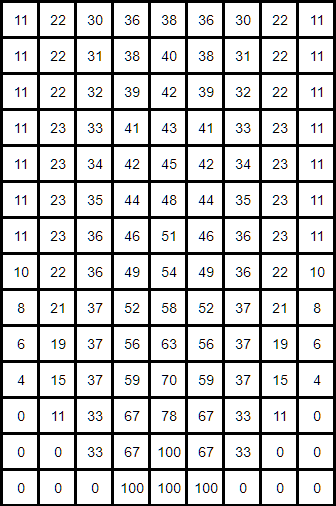
\includegraphics[width=5.09cm]{archivos/fire_whitegrid}
		\caption{Valores resultantes tras convolucionar iterativamente la matriz [\ref{fig:firematrix}] por una matriz de ceros, con valores solo en la fila inferior}
		\label{fig:fire_whitegrid}
	\end{subfigure}
	\begin{subfigure}[b]{0.45\textwidth}
		\centering
		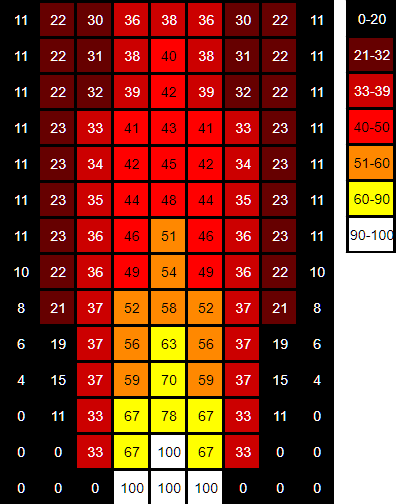
\includegraphics[width=6cm]{archivos/fire_colouredgrid}
		\caption{Efecto resultante de asociar determinados rangos de valores a un set de colores preestablecido}
		\label{fig:fire_colouredgrid}
	\end{subfigure}
\end{figure}

Dado el comportamiento descrito, será necesario realizar los siguientes pasos:
\begin{itemize}
	\item Implementar una forma de realizar degradados (o mapas de color)
	\item Reservar e inicializar una matriz a cero, con valores aleatorios en su fila inferior
	\item Implementar el comportamiento de convolución de la matriz [\ref{fig:firematrix}]
\end{itemize}

\subsection{Implementación}

Para poder crear degradados, se crea la función \emph{GenerateGradient} que dado un conjunto de \emph{ColourStamp} y un tamaño, interpola los valores de colores pasados para generar un degradado continuo en \emph{colourMap}.\\

\begin{lstlisting}[style=C-color, caption={Método para crear gradientes de color},label=cod:generateGradient]
static void GenerateGradient(std::vector<ColourStamp> colours, Pixel* colourMap, int colourMapSize);
\end{lstlisting}

\emph{ColourStamp} (marca de color) es una estructura formada por dos variables: un color y un número decimal (que puede oscilar entre 0 y 1). Este número señala la posición de este color en el gradiente o mapa de color, siendo 0 el inicio y 1 el final. 

\begin{figure}[h]
	\centering
	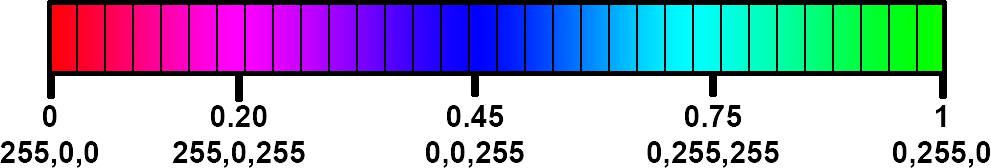
\includegraphics[width=12cm]{archivos/colourGradient}
	\caption{Degradado en 32 celdas dadas 5 marcas de color}
	\label{fig:colourGradient}
\end{figure}

De este modo, si llamamos a la función \emph{GenerateGradient} con los valores para las marcas de color representados en la figura [\ref{fig:colourGradient}] y pasamos un \emph{array} con capacidad para 32 valores, este método producirá un set de colores similar al ilustrado. Esto se hace mediante una interpolación lineal entre los valores que se pasan, creando un degradado de forma progresiva.\\

Una vez tenemos implementado este método, ya podemos crear un degradado de colores de forma sencilla y cómoda, automatizando el proceso de crear un mapa de color para el fuego.\\

Para nuestra implementación, en lugar de asignar a un rango de valores un color específico, asignaremos un color por valor entero. Esto permitirá un resultado más realista, al disponer de una mayor cantidad de colores. Cada celda de nuestra matriz de valores estará formada por un byte. Esto implica que cada celda podrá tener 256 valores distintos, y que por tanto necesitaremos generar un degradado que nos devuelva 256 colores.\\

Creamos un mapa de valores de un byte de tamaño, lo inicializamos a 0 e inicializamos aleatoriamente algunas de las celdas de la fila inferior a su valor máximo (255).\\

\begin{lstlisting}[style=C-color, caption={Creación e incialización del mapa de valores},label=cod:screenMapping,escapechar=|]
screenMapping = new unsigned char[width * height];

for (int i = width * (height - 1), n = width * height; i < n; i++)
{
    if (Fast::Rand() % 10 == 0)|\label{line:fastRand}|
    {
        screenMapping[i] = 255;
    }
}
\end{lstlisting}

Como podemos ver en la línea [\ref{line:fastRand}], hacemos uso de una función propia para la generación de números aleatorios. Esta función está basada en el algoritmo \emph{Xorshift}\footnote{\url{https://en.wikipedia.org/wiki/Xorshift}} de George Marsaglia. La apromaximación usada está basada en una respuesta de \emph{StackOverflow}\footnote{\url{https://stackoverflow.com/questions/1640258/need-a-fast-random-generator-for-c}}.\\

La decisión de usar nuestro propio generador de números aleatorios se debe a que el usualmente provisto por la STL \footnote{\url{https://en.wikipedia.org/wiki/Standard_Template_Library}} es innecesariamente lento y complejo para nuestras necesidades. Para nuestro caso, no necesitamos un algoritmo que pase todos los tests de aleatoriedad\footnote{\url{https://es.wikipedia.org/wiki/Pruebas_de_aleatoriedad}}, con tal de que sea suficientemente "aleatorio al ojo" y sea rápido, nos basta.\\

Una vez hecho esto, tan sólo queda implementar el algoritmo principal, que cree el efecto de fuego sobre el mapa de valores previamente creado, de acorde a la operación descrita en la figura [\ref{fig:firematrix}] y asocie dichos valores con un color generado por la función \emph{GenerateGradient} [\ref{cod:generateGradient}].\\

\begin{lstlisting}[style=C-color, caption={Algoritmo básico de efecto de fuego},label=cod:simpleFire,escapechar=|]
for (int i = width * (height - 1); i >= 0; i--)
{
    int lowerCell = width + i;|\label{line:simpleFire1}|
    int newCellValue = screenMapping[i] = (screenMapping[lowerCell + 1] + screenMapping[lowerCell] + screenMapping[lowerCell - 1]) / 3.0;|\label{line:simpleFire2}|
    pixels[i] = colourMap[newCellValue];|\label{line:simpleFire3}|
}
\end{lstlisting}

En el código [\ref{cod:simpleFire}] podemos  ver el algoritmo de generación de fuego en su forma más simple. Recorremos la pantalla de abajo a arriba y operamos por cada píxel. En la línea [\ref{line:simpleFire1}] obtenemos, para una posición dada en el mapa de valores, la posición del valor inmediatamente por debajo del mismo. Una vez obtenida esta posición, operamos haciendo la media usando su valor y los adyacentes. Guardamos el resultado como nuevo valor y usamos a la vez este nuevo valor para asociar un nuevo color al píxel en pantalla (línea [\ref{line:simpleFire3}]). Los valores más altos (255) representan tonos blancos y/o amarillentos, mientras que los valores intermedios representarán valores rojizos y los valores más bajos tendrán asociados colores más oscuros.\\

El resultado de aplicar este algoritmo resulta en una imagen estática y de aspecto poco realista [\ref{fig:fire_simple}], pero que ya se empieza a parecer al efecto que buscamos.\\

\begin{figure}[h]
	\centering
	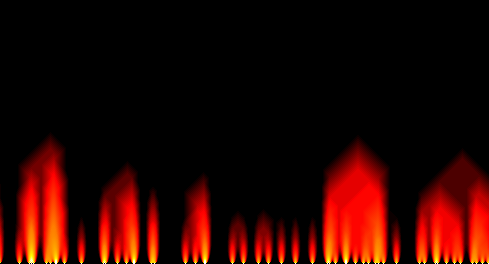
\includegraphics[width=8cm]{archivos/fire_simple}
	\caption{Fuego estático, usando el algoritmo en [\ref{cod:simpleFire}]}
	\label{fig:fire_simple}
\end{figure}

\subsection{Refinamiento}

Una vez tenemos el efecto de fuego a nivel básico, es el momento de iterar sobre la idea y ver cómo mejorarla. A continuación se listan y explican las medidas tomadas, mostradas en el orden en que se aplicaron:

\begin{itemize}
	\item \textbf{Hacer fuego dinámico}: una vez obtenido un fuego estático, era el momento de darle movimiento, y que tuviera un efecto realista. Inicialmente probé con una técnica que se sugería en algunos de los tutoriales que había seguido: en lugar de dibujar el fuego de abajo a arriba, dibujarlo de arriba a abajo y aleatorizar la base, de forma que las variaciones en el fuego derivaran a partir de las variaciones en la base.
	
	El resultado no me dejó convencido. Cuando uno observa un fuego o una llama, la parte más cambiante del fuego no es la base, la base es siempre estable y es la parte superior la que más titila / oscila. Por tanto no tenía para mí sentido generar dinamismo aleatorizando la base.
	
	Una llama se caracteriza a menudo por tener una intensidad variante, y fue esto lo que me decidí por implementar: la base permanecería estable, la llama tendría un factor de aleatoriedad.
	
	Tras un ensayo de prueba y error ajustando valores, y teniendo que retocar la posición y tono de los colores en el gradiente, se llegó al siguiente código \lstinline{(Fast::Rand() % 4 == 0 ? 2 : 0)} que se puede ver aplicado en [\ref{cod:finalFire}]. Básicamente este código altera levemente el valor de intensidad del píxel de forma aleatoria, con un 25\% de posibilidades de que el valor del píxel se vea incrementado. 
	
	El resultado puede verse en [\ref{fig:fire_final}]. La base sobre la que se aplica es la misma que en la figura [\ref{fig:fire_simple}], sin embargo, el resultado resulta más convincente / natural gracias a que se introduce una pequeña aleatoriedad en la intensidad del píxel, introduciendo cierta dispersión.
	
	\item \textbf{Más colores}: una vez tenía el fuego básico creado llegó el momento de ponerse creativo y añadir más degradados, que pudieran ser aplicados para crear fuegos de distintos colores. Al degradado de fuego básico (blanco - amarillo - rojo - negro) se le añadieron dos nuevos degradados, un fuego estilo neón (rosa - verde - azul - negro) y un degradado en blanco y negro (blanco - gris - negro).
	
	Además, el código para generar degradados, que inicialmente estaba en el mismo archivo que el fuego, se separó a su propio archivo y clase. Por último, y en vistas de que el código para crear un degradado ocupaba mucho espacio (debido a la necesidad de definir las marcas de color) y que potencialmente sería reutilizado por otros efectos que usasen degradados, el código se movió a una clase común con inicialización estática. De este modo, desde el inicio de la ejecución están disponibles los vectores de marcas de color necesarios para generar distintos patrones (fuego, neón, blanco y negro, arcoiris...) mediante la función \emph{GenerateGradient}.
	
	\item \textbf{Manipulación del fuego}: una vez teníamos distintos colores, era necesario poder cambiar entre ellos. Fue en este momento cuando se incorporó al motor la capacidad de gestionar entradas de teclado.
	
	Una implementada esta funcionalidad, lo que se hizo fue, al inicio de la ejecución del programa, crear un vector conteniendo patrones de degradado. Luego, al pulsarse una tecla determinada, se actualiza el patrón de degradado en uso al siguiente en el vector.
	
	También se añadió la posibilidad de cambiar levemente la intensidad del fuego, añadiendo la variable \emph{fireIntensity}, cuya aplicación se puede ver en [\ref{fig:fire_final}].
\end{itemize}

\begin{lstlisting}[style=C-color, caption={Algoritmo final de efecto de fuego},label=cod:finalFire]
for (int i = width * (height - 1); i >= 0; i--)
{
    int sum = width + i;
    sum = screenMapping[i] = (screenMapping[sum + 1] + screenMapping[sum] + screenMapping[sum - 1]) / (3.03 + fireIntensity) + (Fast::Rand() % 4 == 0 ? 2 : 0);
    pixels[i] = colourMap[sum];
}
\end{lstlisting}

\begin{figure}[h]
	\centering
	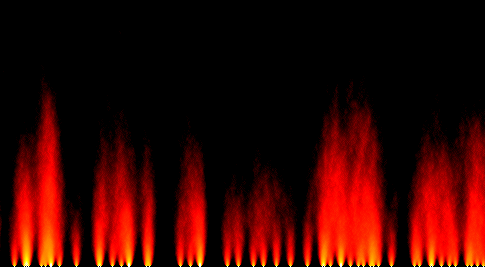
\includegraphics[width=8cm]{archivos/fire_final}
	\caption{Fuego dinámico, con intensidad por píxel aleatorizada}
	\label{fig:fire_final}
\end{figure}

\subsection{Resultado}

A continuación se presenta el resultado final del efecto de fuego: un fuego dinámico, de corte y comportamiento realista, con la posibilidad de cambiar su color y su intensidad.

\begin{figure}[h]
	\centering
	\begin{subfigure}[b]{0.3\textwidth}
		\centering
		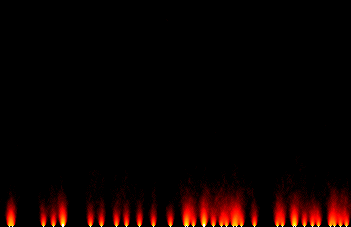
\includegraphics[width=4.5cm]{archivos/fire_final1}
		\caption{Fuego rojo con intensidad mínima}
		\label{fig:fire_final1}
	\end{subfigure}
	\begin{subfigure}[b]{0.3\textwidth}
		\centering
		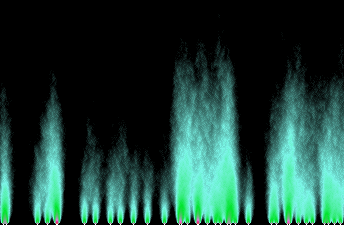
\includegraphics[width=4.5cm]{archivos/fire_final2}
		\caption{Fuego neón con intensidad media}
		\label{fig:fire_final2}
	\end{subfigure}
	\begin{subfigure}[b]{0.3\textwidth}
		\centering
		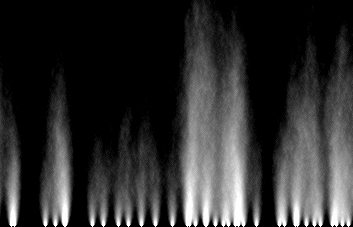
\includegraphics[width=4.5cm]{archivos/fire_final3}
		\caption{Fuego en blanco y negro con intensidad máxima}
		\label{fig:fire_final3}
	\end{subfigure}
\end{figure}

\section{Túnel de puntos} \label{sec:dottunnel}

\subsection{Investigación inicial}

Un efecto también muy común en el mundo de la \emph{demoscene} es el efecto de túnel o vórtice, entre otras causas por su relativa sencillez sumada a su espectacularidad (por la sensación de profundidad y de dinamismo, evocando a escenas futuristas o situadas en el espacio).\\

Es por ello que el efecto de túnel parecía un candidato perfecto para ser el segundo efecto a implementar; más complejo que el efecto de fuego pero aún así sencillo, y con un resultado visual más complejo.\\

Una vez decidido, llegó el momento de recabar información acerca de este efecto y cómo implementarlo. Mi idea inicial era generar un túnel de puntos como el de la figura [\ref{fig:cyberdance}], sin embargo, conforme fui ahondando en mi búsqueda, descubrí que también era un efecto bastante común generar túneles como el que se muestra en la figura [\ref{fig:dane_kefrens}].\\ 

\begin{figure}[h]
	\centering
	\begin{subfigure}[b]{0.45\textwidth}
		\centering
		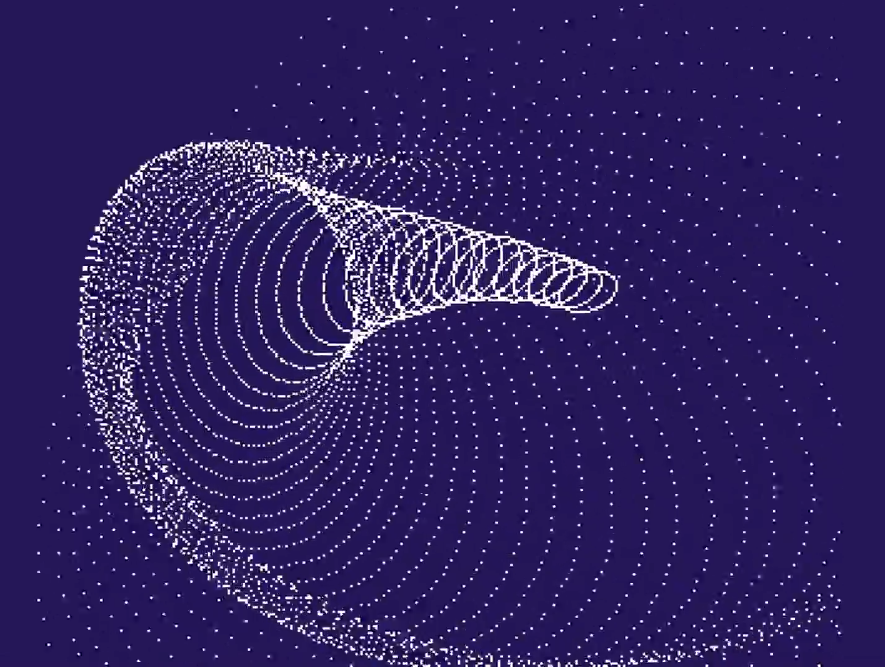
\includegraphics[width=6cm]{archivos/cyberdance}
		\caption{Túnel de puntos - Cyberdance (por Virtual Dreams y Fairlight, 1993) - Fuente: \href{https://www.youtube.com/watch?v=X7sHODKip_c}{YouTube}}
		\label{fig:cyberdance}
	\end{subfigure}
	\begin{subfigure}[b]{0.45\textwidth}
		\centering
		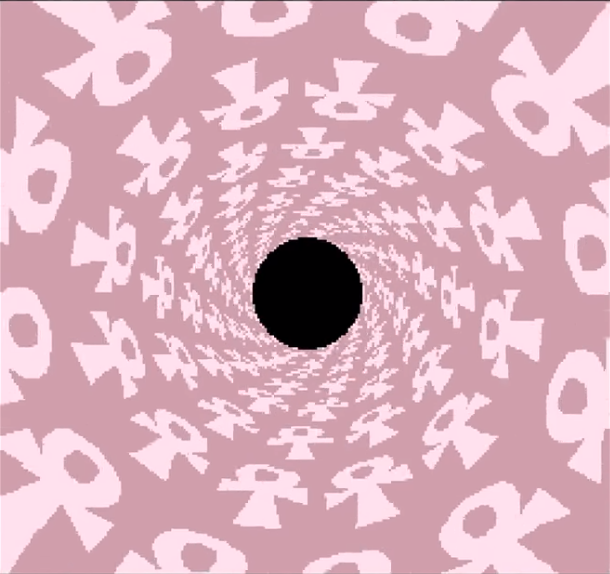
\includegraphics[width=6cm]{archivos/dane_kefrens}
		\caption{Túnel mediante deformación de textura - D.A.N.E (por Kefrens, 1993) - Fuente: \href{https://www.youtube.com/watch?v=ZbPGU5p7O4Y}{YouTube}}
		\label{fig:dane_kefrens}
	\end{subfigure}
\end{figure}

De hecho, de cara a la búsqueda de explicaciones teóricas y detalles de implementación, fue más fácil encontrar información acerca del efecto mostrado en [\ref{fig:dane_kefrens}] que del túnel de puntos. Páginas como \emph{\href{http://benryves.com/tutorials/tunnel}{benryves.com}} o \emph{\href{https://lodev.org/cgtutor/tunnel.html}{lodev.org}} ofrecían tutoriales detallados, en los que se explica paso a paso la base matemática del efecto así como su implementación en código.\\

En resumen, el efecto que se muestra en la figura [\ref{fig:dane_kefrens}] es el resultado de deformar una imagen o una textura de forma que toda la textura tienda hacia un punto central, de modo que se produce una textura circular a partir de un patrón plano. Se deforma la imagen aplicando algo de trigonometría básica. Además, como en el ejemplo de \emph{\href{https://lodev.org/cgtutor/tunnel.html}{lodev.org}}, se pueden usar tablas precalculadas para así evitar tener que realizar operaciones trigonométicas complejas y/o lentas de forma repetida.\\

No fui, sin embargo, capaz de encontrar tutoriales o detalles de implementación para lograr el efecto de la figura [\ref{fig:cyberdance}]. Tras una búsqueda a conciencia con resultado infructuoso, me decidí por implementar este efecto. Mi objetivo con este trabajo no es el de seguir tutoriales ya existentes, si no el de crear efectos visuales partiendo de cero, y guiado por la intuición y la razón. No tiene sentido alguno que trate de implementar un efecto de túnel basado en una textura cuando ya hay tutoriales que desgranan (con detalle y acierto) cómo hacerlo, tanto a nivel matemático como de código.\\

Por tanto, resolví por implementar el efecto de túnel de puntos.

\subsection{Planteamiento formal}

¿Cómo se consigue el efecto de generar un túnel de puntos en movimiento?\\

La respuesta en realidad es bastante sencilla si observamos con atención cualquier demo que implemente este efecto: consiste en la superposición de circunferencias de distintos tamaños y en distintas posiciones. \\

El dibujado de estas circunferencias (o elipses en el caso de la figura [\ref{fig:cyberdance}]) se simplifica a dibujar solo varios puntos pertenecientes a la circunferencia, en lugar de dibujar todo el perímetro. De este modo se consigue un tiempo de dibujado controlable y constante (si decidimos que una circunferencia será representada mediante 16 puntos, se usarán 16 puntos ya sea el radio de la circunferencia 50, 100 o 200 píxeles, de modo que aunque el perímetro aumente, la esfera es representada con una cantidad de puntos constante -eso sí, cada vez más separados entre sí-).\\

Por tanto, será necesario implementar las siguientes funcionalidades:
\begin{itemize}
	\item Capacidad para dibujar un círculo dadas una posición, un radio y por cuantos puntos debe estar formado.
	\item Capacidad para mantener un conjunto de circunferencias simultáneamente
	\item Capacidad para gestionar el ciclo de vida de una circunferencia
	\item Implementar un mecanismo mediante el que el túnel siga una ruta de apariencia natural y fluida
\end{itemize}

\subsection{Implementación}

Empezando por el principio, era necesario poder dibujar circunferencias en pantalla. Estos círculos, además, debían poder variar su posición y tamaño a lo largo del tiempo, por lo que tenía sentido crear una estructura que los representara [\ref{fig:circleuml}].\\

%@startuml
%
%class Circle << (S,#FF7700) Struct >>
%{
%  +float x, y
%  +float radius
%}
%
%hide empty members
%
%@enduml

\begin{figure}[h]
	\centering
	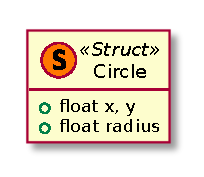
\includegraphics[width=6cm]{archivos/circleuml}
	\caption{Estructura básica de un círculo}
	\label{fig:circleuml}
\end{figure}

Como podemos ver en el código [\ref{cod:drawcircle}], para dibujar una circunferencia, lo que hacemos es ir de \(0\) a \(2 * \pi\). Esto es trazar una circunferencia completa en radianes. Definimos, no obstante, un incremento variable, que depende de la cantidad de puntos que queremos dibujar. De este modo, si queremos dibujar una circunferencia de 4 puntos, este incremento será \((2 \times \pi) \div 4 = \frac{\pi}{2}\), o lo que es lo mismo, dibujaremos de cuarto en cuarto de circunferencia, dibujando así 4 puntos para completar una circunferencia completa.\\

La operación para determinar la posición del punto es muy básica, e implica simplemente un poco de trigonometría. La posición de cada punto de la circunferencia viene determinada por el ángulo (por el coseno del mismo para la coordenada horizontal y por el seno para la coordenada vertical) multiplicado por el radio y sumada la posición del centro de la circunferencia.\\

Una vez obtenida la posición para un punto de la circunferencia, lo dibujamos usando nuestra función del motor para dibujar puntos, que se encarga además de comprobar que el punto esté dentro de los límites de pantalla, y nos permite además pasarle parámetros para el color y el tamaño del punto (blanco y de un píxel para el ejemplo).\\

\begin{lstlisting}[style=C-color, caption={Algoritmo básico de dibujado de circunferencias},label=cod:drawcircle]
void DotTunnelDemo::DrawCircle(const Circle &c)
{
    const float increment = (2 * Fast::PI) / float(pointsPerCircle);
    int x, y;

    for (float angle = 0, n = 2 * Fast::PI; angle < n; angle += increment)
    {
        x = cos(angle) * c.radius + c.x;
        y = sin(angle) * c.radius + c.y;
        
        RenderDot(x, y, Pixel(255), 1);
    }
}
\end{lstlisting}

Una vez podemos dibujar círculos, llega el momento de poder gestionar una serie de círculos y su ciclo de vida (creación, actualizaciones periódicas con radio creciente y destrucción alcanzado un cierto tamaño).\\

Para ello primero debemos preguntarnos, ¿cómo se comporta nuestro túnel? La respuesta es que para la estructura del túnel, lo que queremos es ir añadiendo nuevos círculos al principio del túnel y vamos eliminando los círculos que están al final del túnel cuando alcanzan cierto tamaño. Así pues, esta es una estructura FIFO (\emph{first-in, first-out}) o el primer elemento en crearse es el primer elemento en borrarse. Podríamos pensar que con usar una estructura de cola (\lstinline{std::queue}\footnote{\url{https://en.cppreference.com/w/cpp/container/queue}}) nos bastaría, sin embargo, una cola sólo permite crear un nuevo elemento al final de la estructura y borrarlo al principio, y además no permite el acceso a los elementos intermedios (que nosotros necesitamos para poder actualizarlos).\\

Por suerte, no obstante, hay una estructura similar que cumple todos los requisitos que necesitamos: \lstinline{std::deque}\footnote{\url{https://en.cppreference.com/w/cpp/container/deque}} (\emph{double-ended queue}). Aunque el nombre puede resultar algo extraño (cola con doble final), ¡esta estructura satisface coste constante para todas las operaciones que necesitamos! El coste de la inserción y borrado de elementos son constantes al principio y al final de la cola, y además el acceso aleatorio (acceso a un elemento cualquiera de la cola) es también constante. Por tanto, usaremos esta estructura para contener los círculos que formarán nuestro túnel.\\

\begin{lstlisting}[style=C-color, caption={Inserción y eliminación de círculos},label=cod:populatecirclequeue]
void DotTunnelDemo::PopulateCircleQueue()
{
    if (circles.front().radius > minCircleRadius)
    {
        circles.push_front(defaultCircle);
    }
    if (circles.back().radius > maxCircleRadius)
    {
        circles.pop_back();
    }
}
\end{lstlisting}

Como podemos ver en el código [\ref{cod:populatecirclequeue}], usando esta estructura es muy sencillo añadir y eliminar elementos de nuestro túnel. La lógica que seguimos es: si el último círculo que ha sido añadido alcanza cierto tamaño, entonces añadimos un nuevo círculo al túnel. Del mismo modo, cuando el círculo que más tiempo lleva en la cola alcanza cierto tamaño, es eliminado. Cabe notar que para añadir nuevas circunferencias a la cola, se hace una copia de una instancia que creamos en la inicialización del programa, y que contiene los valores de creación de un círculo por defecto. Además, para que este código funcione correctamente, debe haber al menos un elemento previamente insertado en la cola, es decir, no puede estar vacía. Es por eso que durante la inicialización de la demo también se añade un círculo a la cola, copiado de la instancia por defecto.\\

\begin{lstlisting}[style=C-color, caption={Actualización del túnel},label=cod:updatecirclequeue,escapechar=|]
void DotTunnelDemo::UpdateCircleQueue(float deltaTime)
{
    for (auto c : circles)
    {
        EraseCircle(c);|\label{line:erasecircle}|
    }

    PopulateCircleQueue();

    for (auto &c : circles)
    {
        UpdateCircle(c, deltaTime);|\label{line:updatecircle}|
        DrawCircle(c);
    }
}
\end{lstlisting}

Una vez que podemos dibujar círculos [\ref{cod:drawcircle}] y tenemos una estructura que representa nuestro túnel sobre la que podemos insertar y eliminar elementos [\ref{cod:populatecirclequeue}], llega el momento de dibujar nuestro túnel en pantalla, el proceso es bastante sencillo [\ref{cod:updatecirclequeue}].\\

Lo primero que hacemos es recorrer todos los círculos que conforman el túnel y borrarlos en pantalla, en la línea [\ref{line:erasecircle}]. Es importante notar que esta función no está eliminando los círculos de la cola, si no que simplemente \emph{borra en pantalla}. Internamente esta función llama a la función de dibujado [\ref{cod:drawcircle}] pero con una copia del círculo en color negro. Así, lo que hacemos al inicio de cada actualización es borrar los círculos \emph{que se dibujaron en el fotograma anterior}, previo a la actualización de los valores de los círculos. De este modo, en lugar de tener que poner a negro todos píxeles de la pantalla (que en alta definición son más de un millón), ponemos a negro sólo aquellos píxeles que fueron modificados en el fotograma anterior (que son cientos de píxeles, pero no miles o millones). Al borrar de este modo, se produce una gran optimización.\\

Tras haber borrado la pantalla, llamamos a la función [\ref{cod:populatecirclequeue}], que puede añadir o eliminar círculos del túnel si se cumplen las condiciones necesarias.\\

A continuación, actualizamos (línea [\ref{line:updatecircle}]) y redibujamos todos los círculos en pantalla. Actualmente, la actualización de un píxel es un proceso muy sencillo que consiste simplemente en ir aumentando el radio de cada círculo a lo largo del tiempo, en función de su radio anterior y una velocidad ajustable por el usuario (\lstinline{c.radius += c.radius * deltaTime * radiusVelocity;}).\{\\

El resultado de todo lo aplicado hasta ahora se puede ver en la figura [\ref{fig:basicdottunnel}].\\

\begin{figure}[h]
	\centering
	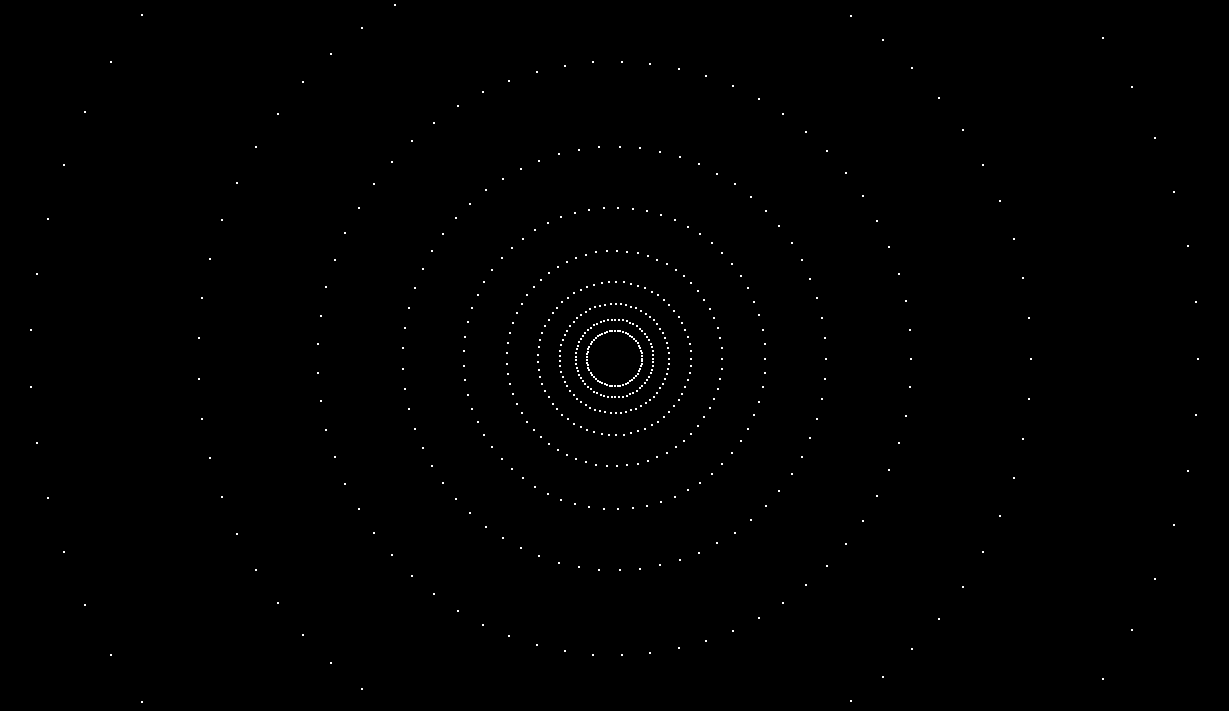
\includegraphics[width=10cm]{archivos/basicdottunnel}
	\caption{Túnel de puntos básico}
	\label{fig:basicdottunnel}
\end{figure}

Ahora todo lo que nos queda por hacer es dotar de movimiento al túnel, es decir, que no sólo los círculos aumenten de radio, si no que su posición también varíe. No obstante, no es necesario modificar la posición de los círculos una vez han sido creados, basta con que el centro de cada círculo esté desplazado en cuanto a posición con respecto al círculo anterior en su momento de creación. En otras palabras, cada círculo se crea en una posición distinta con respecto al punto de creación del círculo anterior, pero el centro del círculo no se modifica posterior a su creación. Aunque pueda resultar curioso, no es necesario mover el centro del círculo una vez creado, basta con ir haciendo el radio progresivamente más grande para crear una sensación de movimiento convincente.\\

Así pues, tan solo necesitamos crear cada círculo con una posición distinta pero coherente con respecto a la anterior, para dar sensación de continuidad. ¿Cómo podemos hacer esto?\\

No podemos decidir las direcciones de forma aleatoria, pues de este modo el movimiento no parecerá coherente. Cabe la posibilidad, no obstante, de seguir direcciones que se deciden aleatoriamente cada cierto tiempo, pero que se mantienen fijas durante un intervalo. Si hacemos esto el movimiento tendría coherencia pero aún así parecería poco natural cada vez que cambiáramos de dirección, pudiéndose producir cambios de dirección bruscos. Una posibilidad ante esto es interpolar la dirección actual con la dirección futura, de modo que los cambios de dirección queden suavizados. Pero aun así surge un problema más, no podemos controlar si el túnel se sale de los límites de la pantalla. Podríamos hacer entonces que si el túnel está cerca del límite de la pantalla, la nueva dirección elegida fuera hacia el centro de la pantalla. Aunque esto podría causar sensación de que cuando el túnel se acerca al límite de la pantalla rebota... Podríamos seguir con este modelo, a partir de direcciones o movimientos aleatorios, pues es factible, pero el código y la cantidad de situaciones con las que hay que lidiar para que el resultado parezca natural aumenta en  complejidad por momentos.\\

Fue por ello que cuando estaba pensando en cómo implementar este efecto, descarté esta opción. Pensando en otras opciones se me ocurrió la que sería la definitiva, construir un camino a partir de un punto que gira en torno a una "órbita" virtual que a su vez "orbita" en torno a otros puntos. Un poco de forma parecida a como orbitan los planetas, que si bien lo hacen bajo rutas perfectamente definidas, las combinaciones de órbitas a distintas velocidades dan resultado a trayectorias coherentes pero difíciles de predecir desde el punto de vista terráqueo [\ref{fig:cassini}].\\

\begin{figure}[h]
	\centering
	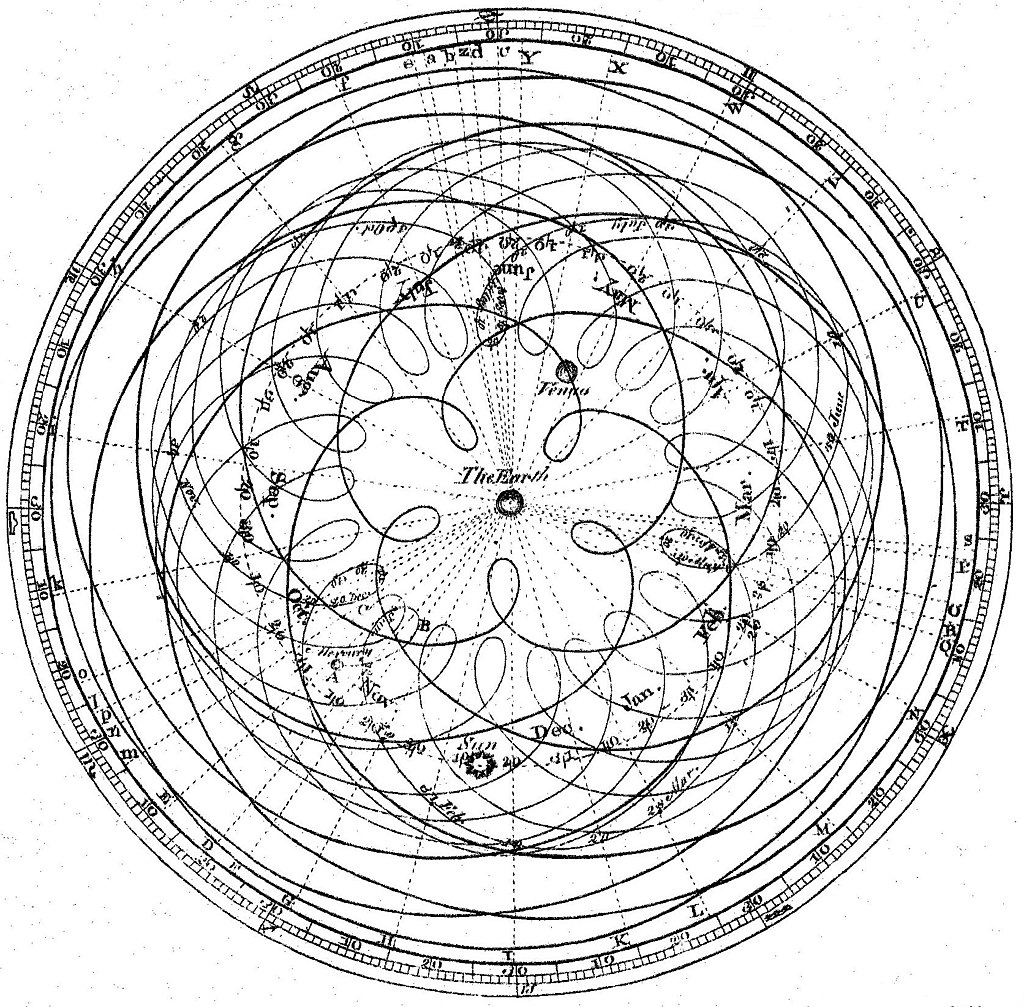
\includegraphics[width=8cm]{archivos/cassini}
	\caption{Órbitas de los planetas vistas desde la Tierra (por Giovanni Cassini) - Fuente: \href{https://es.wikipedia.org/wiki/Teoría_heliocéntrica\#/media/File:Cassini_apparent.jpg}{Wikipedia}}
	\label{fig:cassini}
\end{figure}

Así, con el modelo geocéntrico en mente, me dispuse a crear una clase que fuera capaz de emular este tipo de movimiento: controlado pero difícil de predecir.\\

Todo lo que necesitaba era un algoritmo que me devolviera un valor numérico entre -1 y 1 (al tener un rango controlado el túnel no podría salirse de pantalla) y se calculara como el resultado de la suma de distintos puntos rotando (o como la suma de ondas con distintas frecuencias, según el punto de vista). El resultado fue un algoritmo sencillo pero satisfactorio.\\

\begin{figure}[h]
	\centering
	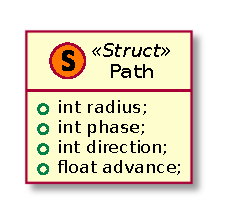
\includegraphics[width=6cm]{archivos/pathuml}
	\caption{Estructura de cada órbita que determina el camino}
	\label{fig:pathuml}
\end{figure}

Como podemos ver en la figura [\ref{fig:pathuml}], creamos una estructura sencilla que nos permite representar un punto orbitando. Un punto orbitando se ve definido por su radio de órbita, su fase (punto inicial en el que comienza a orbitar, la dirección en la que orbita -sentido horario o antihorario- y el avance o camino actual que el punto en órbita ha recorrido. Otras características como la velocidad de órbita se definen de forma global, y no por órbita, para nuestro ejemplo, aunque la velocidad de órbita viene condicionada por el radio de órbita.\\

\begin{lstlisting}[style=C-color, caption={Creación de un camino de turbulencia},label=cod:createturbulencepath,escapechar=|]
void TurbulencePath::CreateTurbulencePath(float pathVelocity, int pathRadius, int pathComplexity)
{
    this->pathVelocity = pathVelocity;
    this->pathRadius = pathRadius;
    this->pathComplexity = pathComplexity;

    for(int i = 0; i < pathComplexity; i++)
    {
        paths.push_back(Path{ |\label{line:createpath}|
                (pathRadius * 2) / (i + 2),
                Fast::Rand() * 2 * Fast::PI,
                i % 2 == 0 ? 1 : -1,
                0});
    }
}
\end{lstlisting}

En el código [\ref{cod:createturbulencepath}] podemos ver cómo podemos inicializar lo que definí como "camino de turbulencia". Para crear un "camino de turbulencia" necesitamos especificar la velocidad global que tendrá el camino, el mayor radio posible que el camino pueda generar, en píxeles, y la complejidad del camino, que es equivalente a la cantidad de órbitas (o ondas) superpuestas que formarán nuestro camino. En la línea [\ref{line:createpath}] podemos ver cómo añadimos caminos, la cantidad que añadimos dependiendo de la complejidad del mismo. Además, el radio de cada órbita depende de su orden (órbita 0 tendrá radio 1 (\(\frac{2}{2}\)), órbita 1 tendrá \(\frac{2}{3}\) del radio, órbita 2 tendrá \(\frac{1}{2}\) (\(\frac{2}{4}\)) del radio...). A continuación definimos la fase de forma aleatoria, la dirección (positiva para órbitas de orden par, negativas para impares) y el avance inicial, que es obviamente 0.\\

\begin{lstlisting}[style=C-color, caption={Actualización de un camino de turbulencia},label=cod:updateturbulencepath,escapechar=|]
void TurbulencePath::UpdateTurbulencePath(float deltaTime, float &pathX, float &pathY)
{
    pathX = 0.f;
    pathY = 0.f;

    for (auto& path : paths)
    {
        path.advance += deltaTime * 0.1;
        float waveFrequence = path.radius * pathVelocity;
        pathX += cos(waveFrequence * path.advance + path.phase);
        pathY += sin(waveFrequence * path.advance + path.phase);
    }

    pathX /= (float)pathComplexity; |\label{line:dividepath}|
    pathY /= (float)pathComplexity;

    pathX *= pathRadius; |\label{line:multiplypath}|
    pathY *= pathRadius;
}
\end{lstlisting}

Ahora llega el momento de ser capaces de actualizar nuestra estructura, como muestra el código [\ref{cod:updateturbulencepath}]. A esta función le pasamos el tiempo transcurrido desde el último fotograma y nos devuelve el punto actual en el que el camino se encuentra. Para ello, por cada camino, actualizamos el avance en función del tiempo y calculamos la frecuencia en función del radio y la velocidad del camino. Una vez hemos sumado todos los caminos, dividimos entre la complejidad (línea [\ref{line:dividepath}]) para normalizar el resultado (de este modo aseguramos que oscila entre -1 y 1). Tras ello, tan solo nos queda multiplicar el resultado normalizado por el radio del camino para obtener el punto en el que nos hallamos actualmente (línea [\ref{line:multiplypath}]).\\

Una vez tenemos nuestro "camino de turbulencia" creado, tan solo tenemos que incorporarlo en nuestro código del túnel e ir actualizándolo periódicamente. Para ello, modificamos la función \lstinline{PopulateCircleQueue()} [\ref{cod:populatecirclequeue}] para que cada vez que añadamos un círculo, desplacemos su centro por la posición actual del "camino de turbulencia".\\

Podemos ver el resultado en la figura [\ref{fig:tunnelwithturbulence}].

\begin{figure}[h]
	\centering
	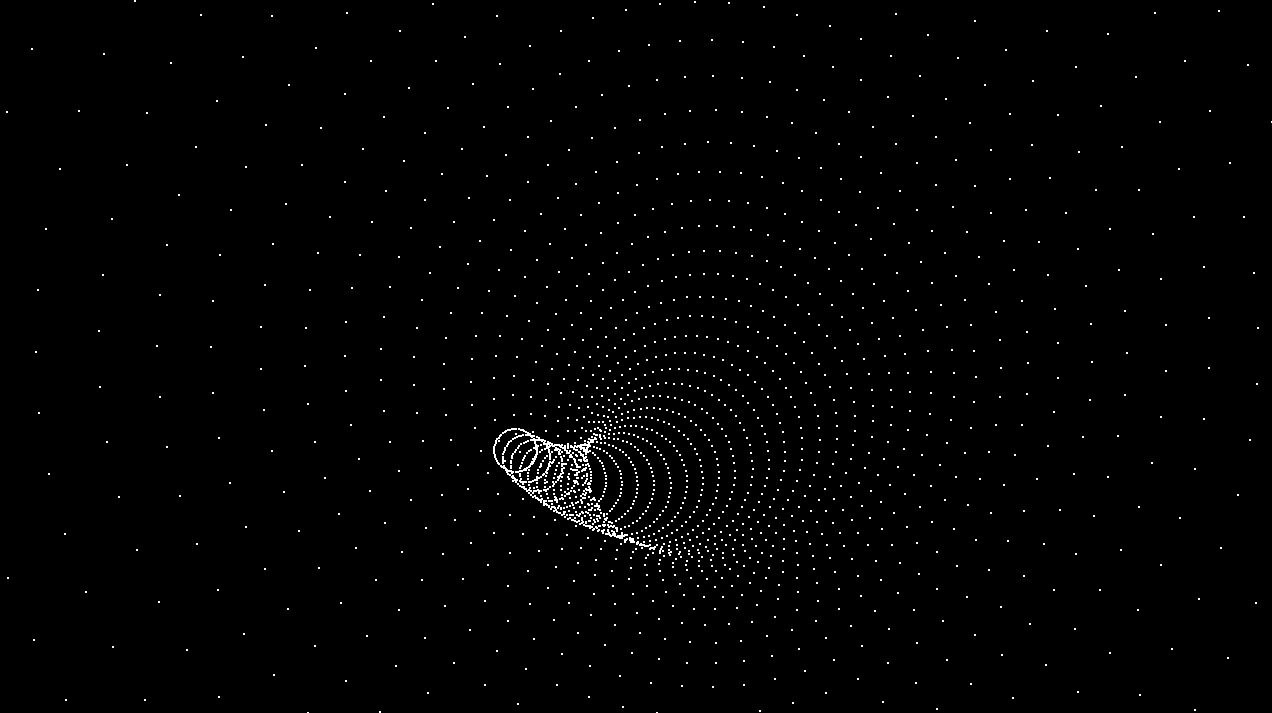
\includegraphics[width=10cm]{archivos/tunnelwithturbulence}
	\caption{Tunel básico siguiendo un camino}
	\label{fig:tunnelwithturbulence}
\end{figure}

\subsection{Refinamiento}

Una vez tenemos nuestro efecto de túnel acabado, llega el momento de iterar sobre la idea para mejorar el resultado, tanto a nivel visual como de rendimiento. A continuación se exponen las medidas que se tomaron:

\begin{itemize}
	\item \textbf{Sustituir operaciones trigonométricas por tablas precalculadas}: como pudimos comprobar con los tests de rendimiento, las operaciones trigonométricas tienen un coste de computación alto. En este efecto hacemos un uso periódico de operaciones de seno y coseno, para calcular la posición de cada punto del túnel, así como para el camino de turbulencia. Si en lugar de usar funciones trigonométricas de forma directa, usamos tablas precalculadas, el coste de estas operaciones pasará a ser el de un acceso constante. No obstante, como todo, usar tablas precalculadas tiene también su coste. La principal ventaja de usar tablas precalculadas es la eficiencia, no obstante lo hacemos al coste de complejidad espacial (tenemos que guardar cada valor precalculado en memoria, y las tablas pueden llegar a ser bastante grandes), pérdida de precisión (al ser valores precalculados, solo podemos acceder a aquellos que hemos calculado, no siendo posible acceder a valores intermedios) y aumento en la complejidad del código (en lugar de pasar un valor en radianes a una función, debemos calcular a partir de un ángulo el índice de acceso a la tabla para el valor que queremos).
	
	Podría parecer, dadas las desventajas listadas, que no vale la pena esta optimización. Esto es siempre una cuestión de interpretación y de límites, y depende de la situación y del sistema en que nos encontremos. En nuestro caso concreto, la memoria no es un limitante (disponemos de gigabytes de memoria RAM) pero sin embargo la CPU sí lo es (tenemos que operar sobre grandes cantidades de valores en intervalos muy cortos de tiempo -cientos o miles de píxeles por fotograma-). Por tanto, vale la pena aumentar la complejidad del código a cambio de que sea notablemente más eficiente.
	
	Como podemos ver en el código [\ref{cod:generatesinetable}], crear una tabla precalculada es más bien sencillo. En este caso, por simplicidad se ha decidido que las tablas se calculan de forma dinámica al inicio de la ejecución de la aplicación, tomando solo así tiempo de cálculo durante la inicialización. No obstante, hubiera sido posible también implementar este mismo mecanismo mediante el uso de \emph{templates} y \emph{constexpr}\footnote{\url{https://en.cppreference.com/w/cpp/language/constexpr}}. De este modo se podría hacer que las tablas se calculasen en tiempo de compilación, embebiéndose la tabla precalculada en el propio código del programa, no tomando así ningún tiempo de cálculo en ejecución. Se ha decido crear las tablas de forma dinámica, no obstante, por simplicidad de código y reducción de los tiempos de compilación.
	
	Así pues, en el código [\ref{cod:generatesinetable}] vemos como para crear una tabla, tan sólo debemos pasarle un tamaño y nos devolverá una tabla del tamaño dado, conteniendo valores incrementales para el seno en una circunferencia completa (de 0 a \(2 \times \pi\) radianes). Hay que tener en cuenta que la precisión de la tabla es equivalente al tamaño de la misma (a mayor tamaño, mayor precisión, pero también ocupa más espacio en memoria y tarda más en calcularse).
	
	En la línea [\ref{line:drawcircle}] podemos ver el resultado de usar nuestras tablas precalculadas en lugar de operaciones trigonométricas de forma directa, como en [\ref{cod:drawcircle}]. Como podemos ver, la complejidad del código aumenta ligeramente, aunque eso sí, a cambio de poder obtener valores de operaciones complejas en tiempo constante. Para ello, necesitamos calcular un factor (línea [\ref{line:indexFactor}]) que nos permita marcar una correspondencia entre el ángulo que queremos y el índice que corresponde en la tabla. Luego, para acceder al valor del coseno (línea [\ref{line:cosinetable}]), multiplicamos el valor del ángulo que queremos por el factor calculado en la línea [\ref{line:indexFactor}]. Convertimos el resultado de esta operación en un entero (el acceso a memoria debe hacerse mediante un valor entero, pues la memoria es discreta, no se puede acceder a "medio bit"), lo que trunca el resultado y lleva a la consiguiente pérdida de precisión. A continuación hallamos el módulo en función del tamaño de la tabla. De este modo, si nos salimos del rango de la tabla, simplemente volvemos a inicio de la misma, de forma circular, por lo que no es posible de forma efectiva salirse de rango.
	
	De este modo, conseguimos una gran optimización (operaciones trigonométricas con coste constante equivalente a un acceso aleatorio). Esta optimización puede no hacerse tan evidente en tiempo de ejecución en esta demo, donde trabajamos con cientos o miles de píxeles, pero sin llegar al orden del millón, pero será crucial en futuros efectos, para conseguir una tasa de actualización de fotogramas estable y fluida.

	\item \textbf{Añadir colores al túnel}: añadir colorido al túnel es muy sencillo, y sin embargo, mejora notablemente el resultado final. Basta con añadir a nuestro modelo de círculo [\ref{fig:circleuml}] un campo para el color, de modo que en lugar de estar predefinido a blanco, el color con el que se dibuja cada círculo dependa del propio círculo. De este modo, podemos crear un degradado de color, como los que ya creamos para el efecto de fuego, y asignar un nuevo color a cada círculo que creamos, basándonos en los valores del degradado. Para este efecto en concreto, hemos decidido crear una gama de colores de efecto \emph{arcoiris}.
	
	\item \textbf{Fundido de entrada y de salida}: en el estado actual de la demo, cuando un círculo se crea aparece de golpe y cuando un círculo se elimina desaparece de golpe. Teniendo en cuenta que actualmente el túnel es fluido tanto a nivel de movimiento (gracias al "camino de turbulencia") como a nivel de color (gracias al uso de un degradado), que los círculos aparezcan y desaparezcan de golpe rompe esta fluidez. Esto es muy sencillo de solucionar, añadiendo un fundido de entrada (opacidad creciente) cuando añadimos un nuevo círculo al túnel y un fundido de salida (opacidad decreciente) cuando estamos cerca de eliminar un círculo. De este modo, basta con crear un método que cumpla la siguiente función:
	
	\begin{itemize}
		\item Cuando un círculo se añade, el valor de la opacidad es 0, y crece gradualmente hasta uno conforme el radio del círculo incrementa
		\item Durante todo el ciclo de vida del círculo la opacidad es 1
		\item Cuando el radio del círculo se acerca al radio máximo (radio que una vez alcanzado, el círculo es eliminado) empezamos a decrementar el valor de la opacidad, de modo que sea 0 cuando el círculo sea eliminado.
	\end{itemize}
	
	De este modo, tan solo tenemos que multiplicar el valor de la opacidad por el color del círculo para conseguir nuestros fundidos de entrada y de salida, suavizando así la creación y eliminación de los círculos.
	
	\item \textbf{Rotación}: actualmente todos los círculos tienen la misma fase inicial (0), de modo que están alineados. Modificando la fase inicial para que se incremente en función del valor del tiempo de vida el círculo, en la función \lstinline{UpdateCircle()}\{, conseguimos que los círculos dejen de estar alineados y tengan una rotación propia, lo que da un cierto efecto de succión o de torbellino al túnel, lo que favorece el resultado visual.
	
	\item \textbf{Control por parte del usuario}: podemos hacer que el túnel sea modificable por el usuario haciendo simplemente que varias variables que ya tenemos se vean alteradas por determinadas entradas de teclado, por ejemplo:
	
	\begin{itemize}
		\item \textbf{Velocidad del túnel}: modificando la variable \emph{radiusVelocity}, que incrementa la velocidad de crecimiento de los círculos
		\item \textbf{Tamaño de los puntos}: nuestra función para dibujar puntos tiene la capacidad para recibir un tamaño, tan solo debemos usar esto en nuestro favor para añadir una variable modificable que contenga el tamaño de los puntos
		\item \textbf{Posición del centro del túnel}: si modificamos el centro del túnel, tenemos la sensación de poder \emph{controlar} el túnel.
	\end{itemize}
	
	De este modo, podemos con modificaciones muy pequeñas hacer que nuestra demo sea ampliamente interactiva. Luego, basta con utilizar la funcionalidad para dibujar texto para comunicar las instrucciones de uso al usuario.
	
\end{itemize}

\begin{lstlisting}[style=C-color, caption={Generación de tablas precalculadas y uso en código}, label=cod:generatesinetable, escapechar=|]
float *Fast::GenerateSineTable(int size)
{
    float *sineTable = new float[size];

    for (int i = 0; i < size; i++)
    {
        float value = (i * 2 * Fast::PI) / size;
        sineTable[i] = sin(value);
    }

    return sineTable;
}

void DotTunnelDemo::DrawCircle(const Circle &c)|\label{line:drawcircle}|
{
    const float increment = (2 * Fast::PI) / float(pointsPerCircle);
    const int indexFactor = mathTableSize / (2 * Fast::PI);|\label{line:indexFactor}|
    int x, y;

    for (float angle = 0, n = 2 * Fast::PI; angle < n; angle += increment)
    {
        x = cosineTable[int(angle * indexFactor) % mathTableSize] * c.radius + c.x; |\label{line:cosinetable}|
        y = sineTable[int(angle * indexFactor) % mathTableSize] * c.radius + c.y;
        
        RenderDot(x, y, Pixel(255), 1);
    }
}
\end{lstlisting}

\subsection{Resultado}

En la figura [\ref{fig:finaltunnel}] podemos ver el resultado final de nuestro túnel. Sigue un camino turbulento, se le aplica un degradado de color, los círculos tienen fundido de entrada y de salida y rotan, creando una sensación de vórtice.\\

Además, el tamaño de los puntos, la posición del centro del túnel y la velocidad del mismo son controlables por el usuario (las instrucciones no se muestran en la figura para no añadir ruido visual al resultado).\\
 
El efecto además usa tablas precalculadas para evitar tener que realizar costosas operaciones trigonométricas (la diferencia en el resultado es apenas visible, aunque prestando atención es posible notar irregularidades entre la distancia de algunos puntos -este error se podría mitigar aumentando el tamaño de la tabla, y por tanto su resolución-). 

\begin{figure}[h]
	\centering
	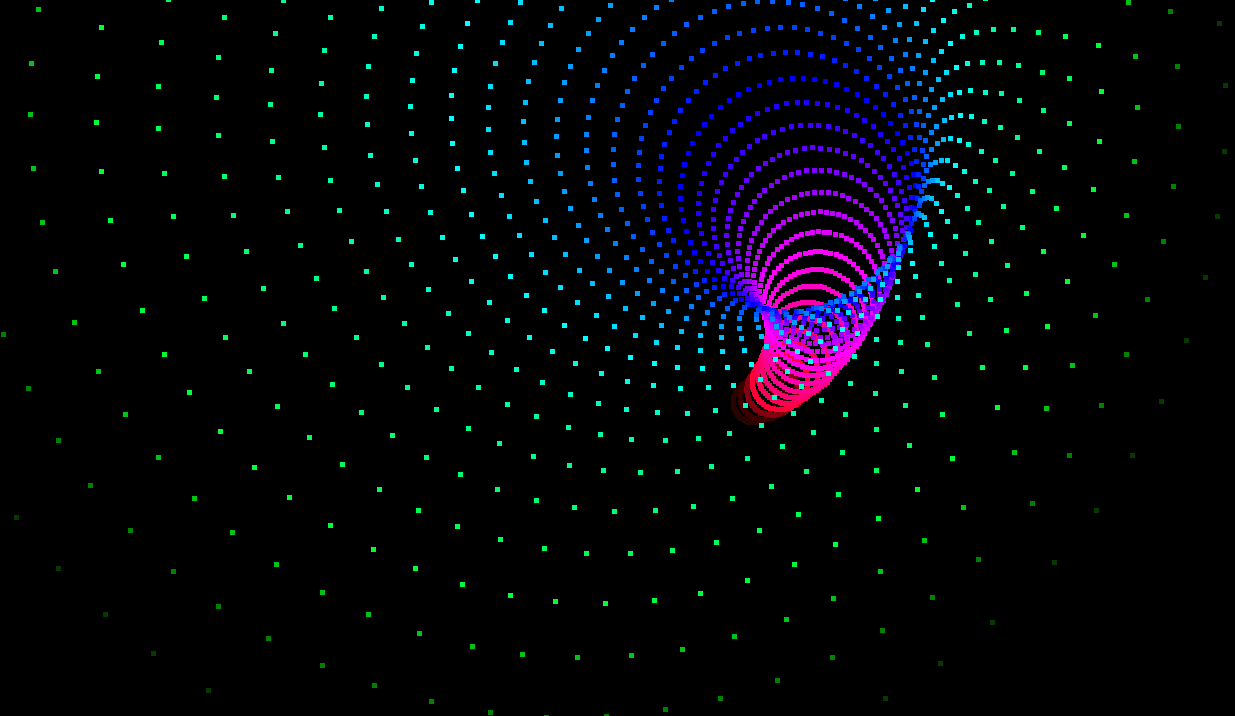
\includegraphics[width=12cm]{archivos/finaltunnel}
	\caption{Túnel final}
	\label{fig:finaltunnel}
\end{figure}

\section{RotoZoom}

\subsection{Investigación inicial}

El efecto de \emph{RotoZoom} es otro de los grandes clásicos de la \emph{demoscene}, y su nombre es bastante autodescriptivo. El efecto de \emph{RotoZoom} consiste en una imagen que se rota y escala en tiempo real. Podemos ver un ejemplo del mismo en la famosa demo \emph{Second Reality} [\ref{fig:second-reality-rotozoom}].\\

Existe amplia documentación para la implementación de este efecto, que además, es muy sencillo, pues se trata simplemente de transformaciones geométricas sencillas en el espacio 2D, dónde el grueso del algoritmo reside en transformar coordenadas en función de una rotación y escala variables.\\

\begin{figure}[h]
	\centering
	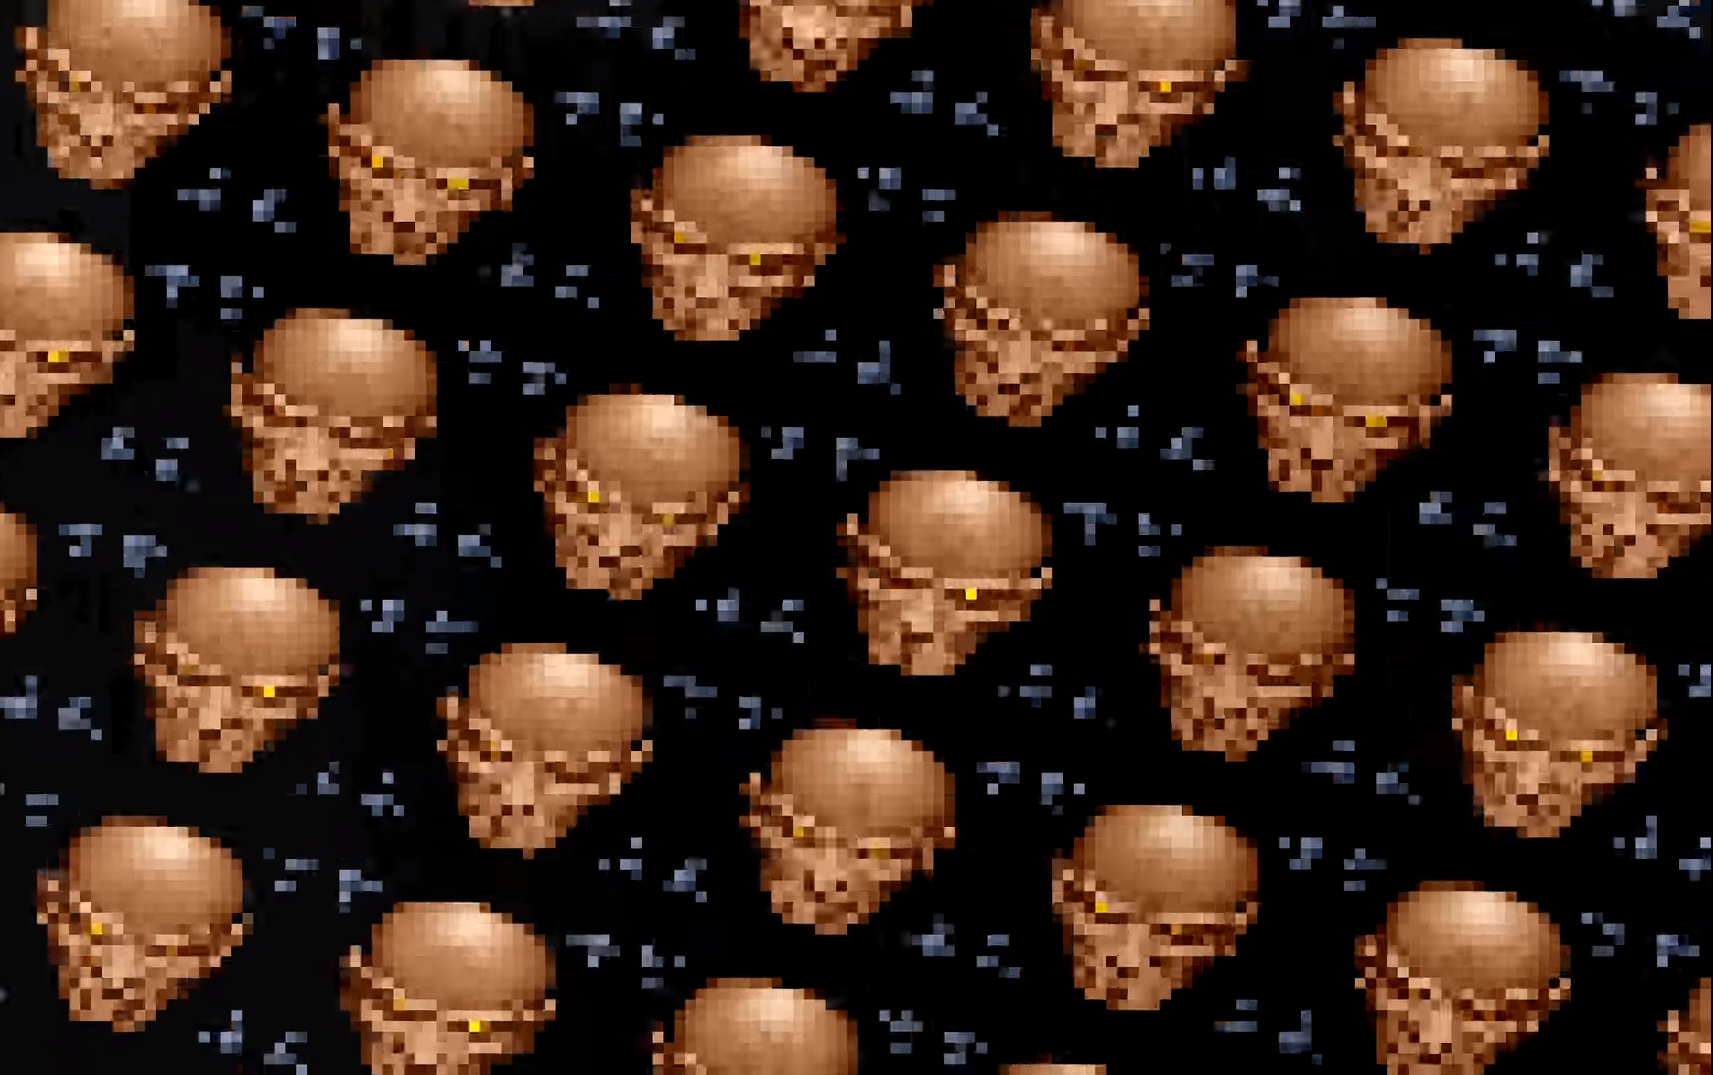
\includegraphics[width=8cm]{archivos/second-reality-rotozoom}
	\caption{Efecto de RotoZoom - Second Reality (by Future Crew) - Fuente: \href{https://www.youtube.com/watch?v=rFv7mHTf0nA&t=5m6s}{YouTube}}
	\label{fig:second-reality-rotozoom}
\end{figure}

\subsection{Planteamiento formal}

En la figura [\ref{fig:transform}] podemos ver las tranformaciones necesarias en el espacio bidimensional para escalar, rotar y trasladar un vector o un punto. Además, se dan también las operaciones matématicas necesarias para hacerlo. Aparece para cada transformación, en rojo el vector inicial y en granate el vector transformado. El orden de las operaciones de escalado y rotación en el ejemplo son intercambiables, es decir, el resultado de la transformación no se verá alterado por qué operación se realice antes. La traslación, no obstante, siempre debe ser la última operación que se realice (ya que el escalado y la rotación son consistentes cuando se realizan en torno al origen, pero no son conmutativas si el centro se ve desplazado).\\

\begin{figure}[h]
	\centering
	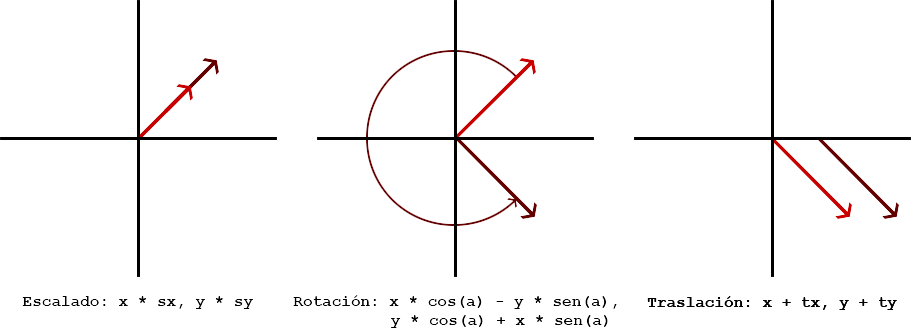
\includegraphics[width=14cm]{archivos/transform}
	\caption{Escalado, rotación y traslación en el espacio 2D}
	\label{fig:transform}
\end{figure}

El algoritmo principal para realizar este efecto será, por tanto, sencillo. No obstante, debemos tener algo en cuenta. Este algoritmo lo aplicaremos sobre una \textbf{imagen} y actualmente, no tenemos modo alguno de cargar imágenes en nuestras demos, por lo que tendremos que añadir esta funcionalidad.\\

Por tanto, deberemos seguir los siguientes pasos:
\begin{itemize}
	\item Implementar un modo de cargar imágenes en nuestra demo
	\item Realizar transformaciones geométricas sencillas para emular el efecto de rotación y escalado
\end{itemize}

\subsection{Implementación}

Lo primero que necesitamos hacer es tener un modo de cargar imágenes en nuestro sistema. Siguiendo con la filosofía de este trabajo, intentamos minimizar el uso de librerías externas al máximo, intentando implementar desde cero todo aquello que esté dentro de un ámbito razonable. La \emph{standard library} de C++ nos ofrece funcionalidades para manejar ficheros binarios, por lo que podremos usarlas para hacer nuestro trabajo más sencillo. No obstante, necesitaremos interpretar el fichero cargado en memoria para que una cadena de bytes en memoria pase a convertirse en una imagen que podemos manipular.\\

Es por ello que lo primero que cabe preguntarse es: ¿qué formato de imagen debemos emplear? Para no salir del ámbito de este trabajo, debemos elegir un formato que sea sencillo de leer y manipular, y este es sin duda, BMP, un formato de imagen sin transparencia ni compresión. En Wikipedia se ofrece una explicación en profundidad del formato BMP \footnote{\url{https://en.wikipedia.org/wiki/BMP_file_format}}, que nos será muy útil para saber cómo interpretarlo.\\

Estas son las consideraciones que tendremos en cuenta para nuestra cargar de imágenes en BMP, a partir de un archivo binario cargado en memoria:

\begin{itemize}
	\item Necesitamos saber la anchura de la imagen, que se puede encontrar en el byte 18 del fichero BMP y ocupa 4 bytes, en \emph{little-endian}
	\item Necesitamos saber la altura de la imagen, que se puede encontrar en el byte 22 del fichero BMP y ocupa 4 bytes, en \emph{little-endian}
	\item Asumimos que la profundidad de color será de 24 bits por píxel (1 byte por color)
	\item Asumimos que no hay ningún tipo de compresión
	\item En el formato BMP cada fila de la imagen está alineada a 32 bits
	\item En el formato BMP, la imagen está guardada de abajo a arriba y de izquierda a derecha (es decir, por filas, empezando en la inferior)
\end{itemize}

%@startuml
%
%class FileLoader
%{
%  +OpenBinaryFile(in path, out file, out size)
%  +CloseBinaryFile(in file)
%}
%
%class BMP
%{
%  +OpenRGBImage(in path, out image, out width, out height)
%  +CloseRGBImage(in image)
%  -CharToInt(in pointerToCharArray)
%}
%
%hide empty members
%
%BMP -> FileLoader : "uses"
%
%@enduml

\begin{figure}[h]
	\centering
	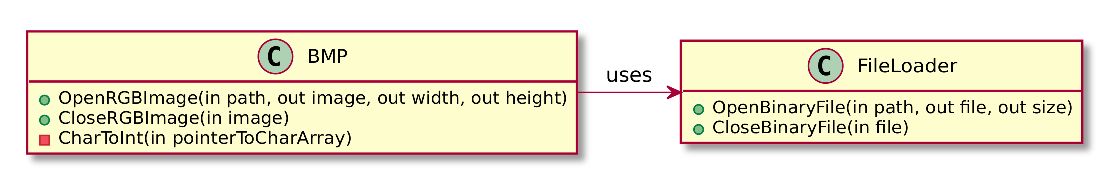
\includegraphics[width=14cm]{archivos/bmpuml}
	\caption{Diagrama del sistema para cargar imágenes}
	\label{fig:bmpuml}
\end{figure}

Como podemos ver en la figura [\ref{fig:bmpuml}], nos ayudaremos de una clase a la que hemos llamado \emph{FileLoader} a la que simplemente pasaremos una cadena de texto con la ubicación de la imagen que queremos abrir y nos devolverá una copia del fichero (como una cadena de bytes \lstinline{unsigned char *}\{) y el tamaño en bytes del mismo. Para realizar estas operaciones, nos ayudamos de la librería \emph{fstream} de la \emph{standard library}.\\

Nuestra clase principal, \emph{BMP} [\ref{fig:bmpuml}], convertirá la cadena de bytes (\lstinline{unsigned char *}\{) que recibe del \emph{FileLoader} en una cadena de píxeles (\lstinline{Pixel *}\{) usable por nuestras demos.\\

\begin{lstlisting}[style=C-color, caption={Código para cargar una imagen BMP en nuestro sistema}, label=cod:openrgbimage, escapechar=|]
void BMP::OpenRGBImage(const char *path, Pixel *&image, int &width, int &height)
{
    unsigned char *imageBinary = nullptr;
    unsigned int imageSize;

    FileLoader::OpenBinaryFile(path, imageBinary, imageSize);

    width = CharToInt(imageBinary + 18);  //Offset where width info is in BMP format
    height = CharToInt(imageBinary + 22); //Offset where height info is in BMP format
    image = new Pixel[width * height]; |\label{line:pixeltexture}|

    for (int j = 0; j < height; j++)
    {
        for (int i = 0; i < width; i++)
        {
            //The first part of the index "(imageSize - (j + 1) * width * 3) + i * 3" 
            //draws the image inverted in the Y axis
            //The second part of the index "- ((width * 3) % 4) * j" 
            //adds the corresponding offset (in the BMP format
            //All rows are 32 bit aligned)
            int index = (imageSize - (j + 1) * width * 3) + i * 3 - ((width * 3) % 4) * j; |\label{line:bmpindex}|
            image[j * width + i] = Pixel(imageBinary[index + 2], imageBinary[index + 1], imageBinary[index]);
        }
    }

    FileLoader::CloseBinaryFile(imageBinary);
}
\end{lstlisting}

Aunque el código [\ref{cod:openrgbimage}] pueda parecer algo complejo, en realidad es bastante sencillo. Una vez tenemos un puntero a nuestro archivo binario, que sabemos que será un fichero BMP, lo primero que hacemos es obtener la altura y anchura de la imagen a leer. Como sabemos la posición en la que se encuentran la anchura y la altura, dado que vienen especificadas por el formato, tan solo tenemos que acceder directamente a la posición donde se encuentran los bytes que nos interesan e interpretarlos. Es por ello que necesitamos una función que sea capaz de, a partir de una dirección de memoria dada, leer 4 bytes que representan un entero de 32 bits en \emph{little-endian}\footnote{\url{https://en.wikipedia.org/wiki/Endianness\#Little-endian}} y devolver como resultado un entero [\ref{cod:chartoint}]. Logramos este resultado mediante el uso de operaciones a nivel de bit, creando una correspondencia byte a byte entre nuestra cadena de bytes y nuestro entero.\\

\begin{lstlisting}[style=C-color, caption={Código para convertir una cadena de 4 bytes en un entero de 32 bits}, label=cod:chartoint]
int BMP::CharToInt(unsigned char *p)
{
    int number = 0;

    number = p[0];
    number = number | p[1] << 8;
    number = number | p[2] << 16;
    number = number | p[3] << 24;

    return number;
}
\end{lstlisting}

Una vez hemos obtenido de las cabeceras de nuestro fichero BMP la anchura y altura de la imagen a procesar, en píxeles, podemos calcular el tamaño de nuestra textura e inicializar una textura formada por nuestros píxeles, como podemos ver en la línea [\ref{line:pixeltexture}]. Ahora, debemos rellenar nuestra recién creada textura de un modo que sea fácilmente manipulable en nuestro sistema. Para ello, tenemos que tener en cuenta que el formato BMP incluye la información fila a fila de abajo arriba, por lo que nosotros tendremos que invertirla, para poder tratar nuestra imagen de forma más cómoda, de arriba abajo. Además, tenemos que tener en cuenta que los píxeles están alineados a 32 bits por cada fila. Como podemos ver en la figura [\ref{fig:pixelalignment}], en una imagen de 5x4 píxeles, el formato BMP incluiría un byte extra por fila, de modo que las filas estén siempre alineadas a 32 bits. En la figura [\ref{fig:pixelalignment}], cada celda representa un byte, cada grupo de color (gris o blanco) representa un píxel (tres bytes) y el color rojo representa los bytes añadidos al final de cada fila para que la memoria esté alineada a 32 bits (4 bytes).\\

\begin{figure}[h]
	\centering
	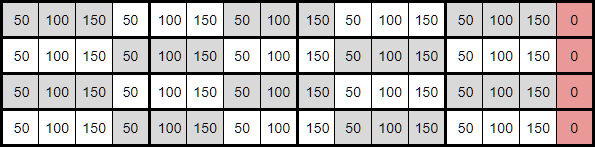
\includegraphics[width=12cm]{archivos/pixelalignment}
	\caption{Representación de los píxeles para una imagen 5x4 en BMP}
	\label{fig:pixelalignment}
\end{figure}

Es por ello que si bien rellenamos nuestra textura de arriba abajo, de izquierda a derecha y de forma lineal, en la línea [\ref{line:bmpindex}] calculamos un índice que accede a nuestro fichero BMP de abajo arriba, de izquierda a derecha y saltando al final de cada  fila (evitando introducir datos basura que se usan para mantener el alineamiento por fila).\\

Tras ello, nos aseguramos de liberar la memoria correspondiente y ¡ya hemos convertido nuestra imagen BMP a un formato manejable en nuestras demos!\\

Ahora tan solo queda implementar el algoritmo de \emph{RotoZoom}, lo cual resulta bastante trivial, como podemos ver en el código [\ref{cod:drawrotozoom}]. Para hallar la posición de la textura que corresponde a nuestro píxel, aplicamos primero una rotación, tras ello un escalado y por último, sumamos un desplazamiento. Cabe denotar que para mantener la coherencia de los resultados, nos quedamos con el valor absoluto de la transformación y le aplicamos el módulo en función del tamaño de la textura, para evitar que nuestro píxel se salga de los límites de la textura.\\

\begin{lstlisting}[style=C-color, caption={Dibujar un píxel cuya textura se desplaza en función de un ángulo, una escala y una traslación}, label=cod:drawrotozoom]
void RotoZoom::DrawPixel(int x, int y, int offsetX, int offsetY, int angle, float scale)
{
    int texX = Fast::Abs(int((x * cos(angle) - y * sin(angle)) * scale + offsetX)) % texWidth;
    int texY = Fast::Abs(int((y * cos(angle) + x * sin(angle)) * scale + offsetY)) % texHeight;

    pixels[y * width + x] = texture[texY * texWidth + texX];
}
\end{lstlisting}

Una vez aplicada esta transformación, ¡nuestro efecto de \emph{RotoZoom} está acabado! Y con una tasa de fotogramas de nada más y nada menos que \textbf{5 fotogramas por segundo}...

\subsection{Refinamiento}

Como vimos en los tests de rendimiento y como hemos mencionado en el análisis del efecto del Túnel de puntos, las operaciones con funciones matemáticas son costosas. \textbf{Muy costosas}. Si operamos tan solo con unos pocos píxeles no hay problema, pero si debemos iterar sobre cada uno de los píxeles en pantalla, que en nuestro caso son más de un millón... resulta inviable.\\

El primer cambio que podemos hacer, si nos fijamos en el código [\ref{cod:drawrotozoom}], es extraer el resultado del seno y el coseno a una variable, ya que se realiza la misma operación dos veces. Únicamente hacer esto ya duplicará la velocidad de fotogramas, a 10 fotogramas por segundo, lo cual sigue siendo inaceptable.\\

Por suerte, y con previsión, ya hemos implementado un método para generar tablas precalculadas [\ref{cod:generatesinetable}]. Si en lugar de usar funciones matemáticas usamos valores precalculados, nuestra tasa de fotogramas aumenta a \textbf{28 por segundo} en modo \emph{debug} y \textbf{40 fotogramas por segundo} en modo \emph{release}, las cuales ya se pueden considerar tasas de fotogramas aceptables, dado que el ojo humano percibe continuidad a partir de algo más de 12 fotogramas por segundo\footnote{\url{https://es.wikipedia.org/wiki/Fotogramas_por_segundo}}.\\

Ahora que tenemos una tasa de fotogramas adecuada y estable, llega el momento de crear una sensación de movimiento que parezca aleatorio pero continuo y fluido... por suerte, este también es un problema que se repite, pues es el mismo problema que teníamos con la ruta que debía seguir el "túnel de puntos". Así que podemos reutilizar la solución, ajustando valores. Así pues, creamos un "camino de turbulencia" que controlará los valores \emph{x} e \emph{y} de nuestra traslación y otro que controlará los valores del ángulo y la escala.\\

De este modo, las transformaciones que aplicamos sobre nuestros píxeles tendrán un efecto continuo y fluido, pero con una ruta impredecible.\\

\subsection{Resultado}

\begin{figure}[h]
	\centering
	\begin{subfigure}[b]{0.48\textwidth}
		\centering
		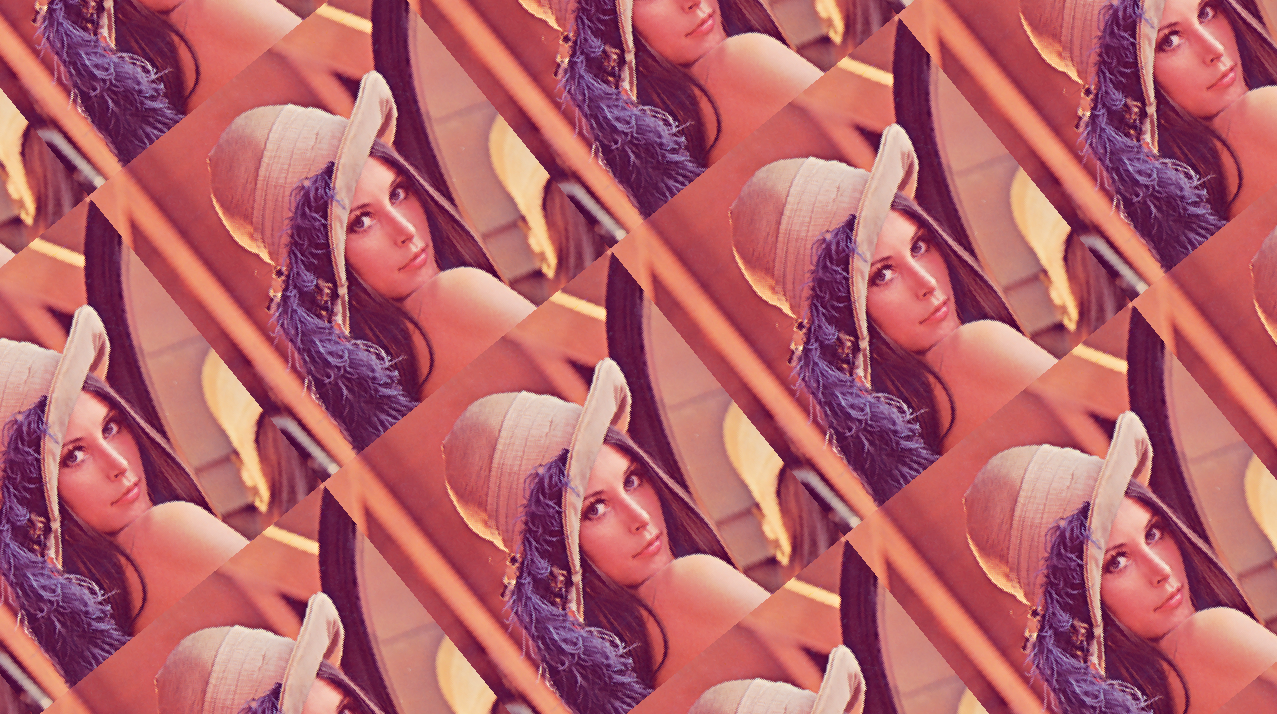
\includegraphics[width=7.5cm]{archivos/rotozoom1}
		\label{fig:rotozoom1}
	\end{subfigure}
	\begin{subfigure}[b]{0.48\textwidth}
		\centering
		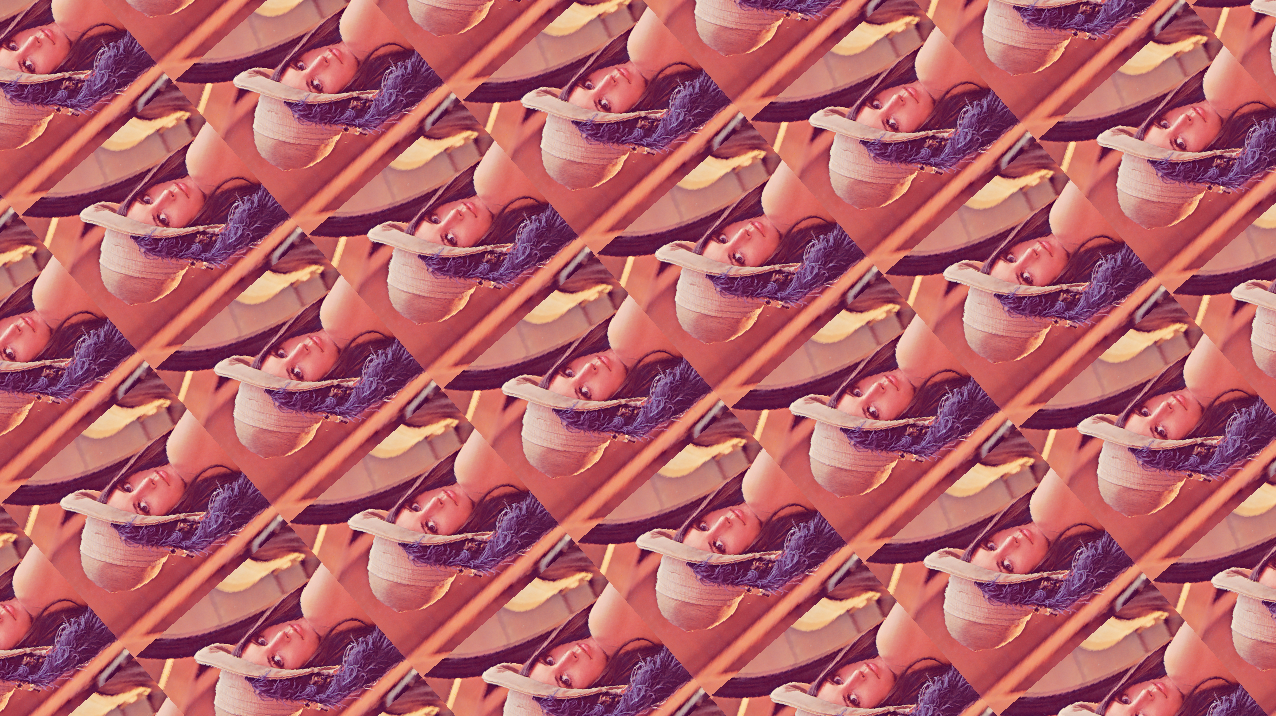
\includegraphics[width=7.5cm]{archivos/rotozoom2}
		\label{fig:rotozoom2}
	\end{subfigure}
	\caption{RotoZoom en distintos estados}
\end{figure}

\section{Deformaciones de imagen}

\subsection{Investigación inicial}

Las deformaciones de imagen son un efecto muy socorrido en el mundo de la \emph{demoscene} y de formas muy distintas. Efectos de lupa y/o deformaciones de lente, estiramientos, efectos de muelle o rebote, torsiones, espirales, en túnel...\\

Sólo implementar todas las diferentes propuestas y efectos de deformaciones de imagen podría llevar su propia investigación y trabajo. No obstante, el denominador común de muchas de estas transformaciones es que usan operaciones trigonométricas, y al final no dejan de ser combinaciones  distintas de senos y cosenos a los que se aplican distintos parámetros.\\

Es por ello que para las deformaciones de imagen, nos centraremos en las deformaciones de onda, pues muchos de los efectos que podemos encontrar en demos parten de estas mismas bases matemáticas.\\

\subsection{Planteamiento formal}

En la figura [\ref{fig:wavefunction}] podemos ver la ecuación de la onda, donde \(A\) es la amplitud de la onda, lo que en nuestro efecto se traducirá en la altura máxima y mínima de nuestra onda, en píxeles. \(f\) se corresponde con la frecuencia de la onda (cuántas veces por segundo se completa un ciclo de onda), \(\lambda\) es la longitud de onda (distancia entre dos crestas consecutivas de la onda), \(t\) es el tiempo transcurrido y \(\phi\) es la fase inicial (o desplazamiento inicial con respecto al origen).\\

\begin{figure}[h]
	\centering
	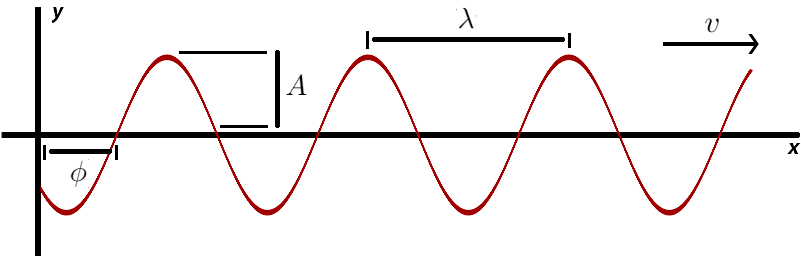
\includegraphics[width=13cm]{archivos/wave}
	\resizebox{6cm}{!}{\(A \sin{(2 \pi v t + \phi)}, v = f \lambda\)}
	\caption{Representación gráfica de la onda y su ecuación}
	\label{fig:wavefunction}
\end{figure}

Además, podemos distinguir dos tipos distintos de onda, dependiendo de su forma de movimiento. Una \textbf{onda transversal} es aquella en la que la dirección de movimiento es perpendicular a la dirección de oscilación\footnote{\url{https://es.wikipedia.org/wiki/Onda_transversal}} mientras que una \textbf{onda longitudinal} es aquella en la que la dirección de movimiento es paralela a la dirección de oscilación\footnote{\url{https://es.wikipedia.org/wiki/Onda_longitudinal}}. Por ejemplo, un muelle es un ejemplo de onda longitudinal, pues oscila (rebota) en la misma dirección en la que se mueve, mientras que las ondas que se producen al lanzar una piedra en el agua son un buen ejemplo de onda transversal (pues mientras que el agua oscila de arriba abajo, la onda avanza en línea recta, perpendicular a su oscilación).\\

En la figura [\ref{fig:transversalwave}] podemos ver la fórmula de la onda transversal. Tiene sentido que el avance de esta onda sea perpendicular a su dirección de oscilación, dado que como se muestra en la figura, el valor de \(y\) depende de \(x\), por lo que el valor en el eje \(y\) depende del valor en el eje perpendicular al mismo. Esto mismo se extrapola a la figura [\ref{fig:longitudinalwave}], dónde el avance de la onda en \(y\) depende de \(y\), por lo que la dirección de propagación coincide con la dirección de oscilación.\\

\begin{figure}[h]
	\centering
	\begin{subfigure}[b]{0.45\textwidth}
		\centering
		\resizebox{4cm}{!}{\(y = A \sin{(2 \pi \frac{x}{\lambda} + \phi)}\)}
		\caption{Onda transversal}
		\label{fig:transversalwave}
	\end{subfigure}
	\begin{subfigure}[b]{0.45\textwidth}
		\centering
		\resizebox{4cm}{!}{\(y = A \sin{(2 \pi \frac{y}{\lambda} + \phi)}\)}
		\caption{Onda longitudinal}
		\label{fig:longitudinalwave}
	\end{subfigure}
\end{figure}

Con todo lo visto, para poder crear nuestro efecto de deformaciones de imagen necesitaremos:

\begin{itemize}
	\item Implementar un modo de aplicar deformaciones a nuestra imagen 
	\item Implementar un sistema que permita manejar con facilidad distintas ondas	
	\item Implementar distintos tipos de ondas, con distintos parámetros
\end{itemize}

\subsection{Implementación}

Como podemos ver en el código [\ref{cod:drawdeformation}], empezamos por definir una función delegada que nos devuelva un valor entero en función del valor de entrada, que serán las coordenadas \emph{x} e \emph{y}. De este modo, podemos definir nuestro comportamiento de deformación encapsulado en sus propios métodos, generando un código más fácil de mantener y un programa fácilmente modificable en tiempo de ejecución.\\

\begin{lstlisting}[style=C-color, caption={Dibujado de un pixel aplicando una función que modifica el acceso a textura}, label=cod:drawdeformation]
typedef int (Deformations::*delegate)(int, int);

void Deformations::DrawPixel(int x, int y, float deltaTime, delegate xModifier, delegate yModifier)
{
    int newX = (this->*xModifier)(x, y) % texWidth;
    int newY = (this->*yModifier)(x, y) % texHeight;

    pixels[y * width + x] = texture[newY * texWidth + newX];
}
\end{lstlisting}

Tras ello, definimos diversos métodos que apliquen nuestras funciones de onda, tanto para \emph{x} como para \emph{y}. En el código [\ref{cod:xmodifiers}] podemos ver los modificadores que definimos para \emph{x}. Definimos así un método por defecto que simplemente devuelve la variable sin modificar (por si no queremos aplicar deformación en absoluto o queremos no aplicar transformación en un eje). Tras ello, definimos un método para generar ondas transversales (como podemos ver, la \emph{x} depende de la \emph{y}) y un método para generar ondas longitudinales (donde \emph{x} depende de sí misma). La variable \emph{k} corresponde al número de ondas (\(k = \frac{2 \pi}{\lambda}\)). Además, en nuestro caso sumamos una fase inicial variable, que depende del tiempo (multiplicado por una constante definida por el usuario), de modo que se aplique un desplazamiento incremental a la deformación, generando sensación de movimiento.\\

\begin{lstlisting}[style=C-color, caption={Funciones de deformación en X}, label=cod:xmodifiers]
int Deformations::DefaultXModifier(int x, int y)
{
    return x;
}

int Deformations::TransversalWaveXModifier(int x, int y)
{
    return x + amplitude * sineTable[(y * k + int(accumulatedTime * c)) % mathTableSize];
}

int Deformations::LongitudinalWaveXModifier(int x, int y)
{
    return x + amplitude * sineTable[(x * k + int(accumulatedTime * c)) % mathTableSize];
}

int Deformations::FlagXModifier(int x, int y)
{
    return x + bigAmplitude * sineTable[(y + int(accumulatedTime * c)) % mathTableSize];
}
\end{lstlisting}

Como podemos ver, ahora usamos tablas precalculadas desde el principio, pues ya hemos demostrado en el efecto anterior que la única forma de obtener una tasa de fotogramas estable y aceptable es mediante el uso de tablas precalculadas. Calculamos el módulo en función del tamaño de la tabla para asegurarnos de no salirnos de los límites de la misma.\\

Como podemos ver en el código [\ref{cod:xmodifiers}], tenemos un último método al que hemos llamado \emph{FlagModifier}. Esta función ha sido nombrada por el resultado visual que produce, en lugar de haberse elegido su nombre por el tipo de onda que es. Usamos como modificador una onda transversal con una amplitud grande y una longitud de onda también grande (\emph{k} se omite, por lo que \(k = 1\), lo que implica que \(\lambda = 2 \pi\)). Esto produce, al aplicarse sobre la imagen, un efecto similar a una bandera ondeando, de ahí el nombre.\\

Una vez hemos definido nuestras funciones de deformación para \emph{x} e \emph{y}, y habiendo ajustado sus valores, podemos combinarlas y usarlas libremente para crear distintos efectos visuales. Para ello, definimos un vector de pares de modificadores (\lstinline{std::vector<std::pair<delegate, delegate>>}\{. Aunque esta expresión parece algo compleja, es realidad su uso es muy sencillo: al tener un vector de pares de modificadores, podemos añadir fácilmente pares de modificadores y alternarlos. De este modo, podemos aplicar modificadores para \emph{x} e \emph{y} y cambiarlos con facilidad en tiempo de ejecución, aplicando simplemente el siguiente par en el vector.\\

\subsection{Resultado}

Podemos apreciar los resultados de aplicar y combinar las distintas deformaciones en la figura [\ref{fig:alldeformations}].

\begin{figure}
	\centering
	\begin{subfigure}[b]{0.48\textwidth}
		\centering
		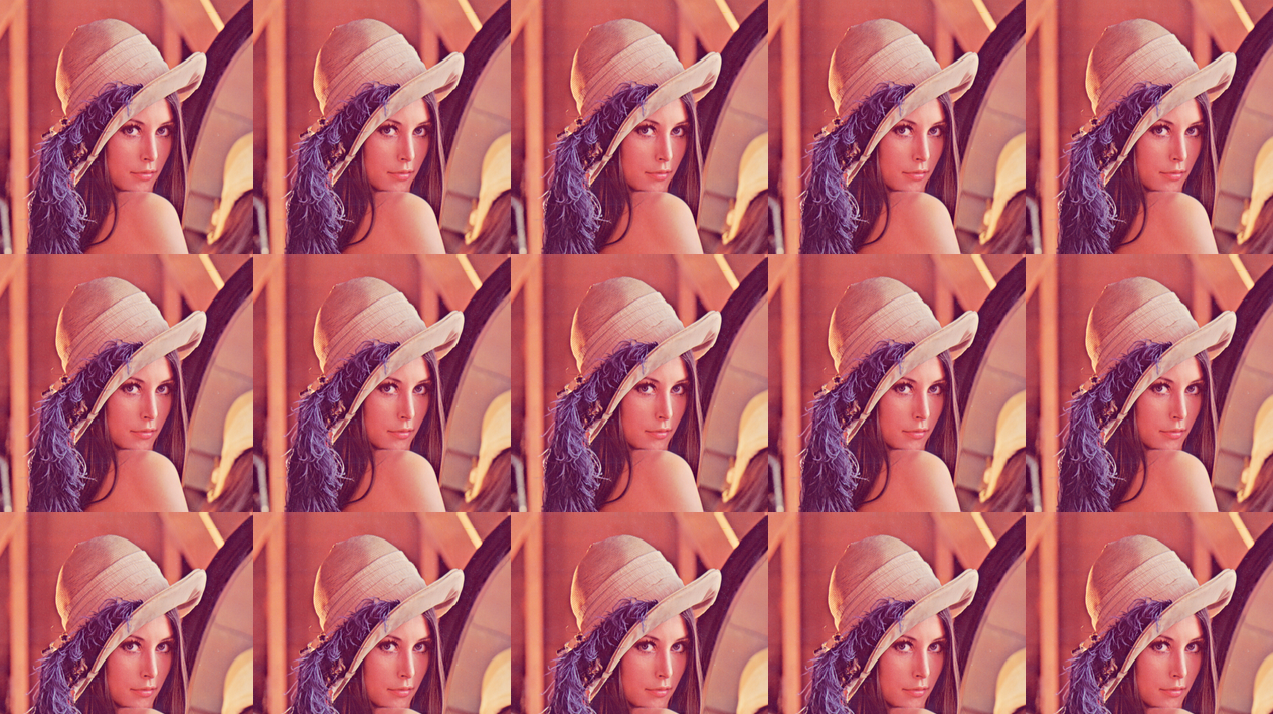
\includegraphics[width=7.5cm]{archivos/deformation1}
		\caption{Sin modificar}
	\end{subfigure}
	\begin{subfigure}[b]{0.48\textwidth}
		\centering
		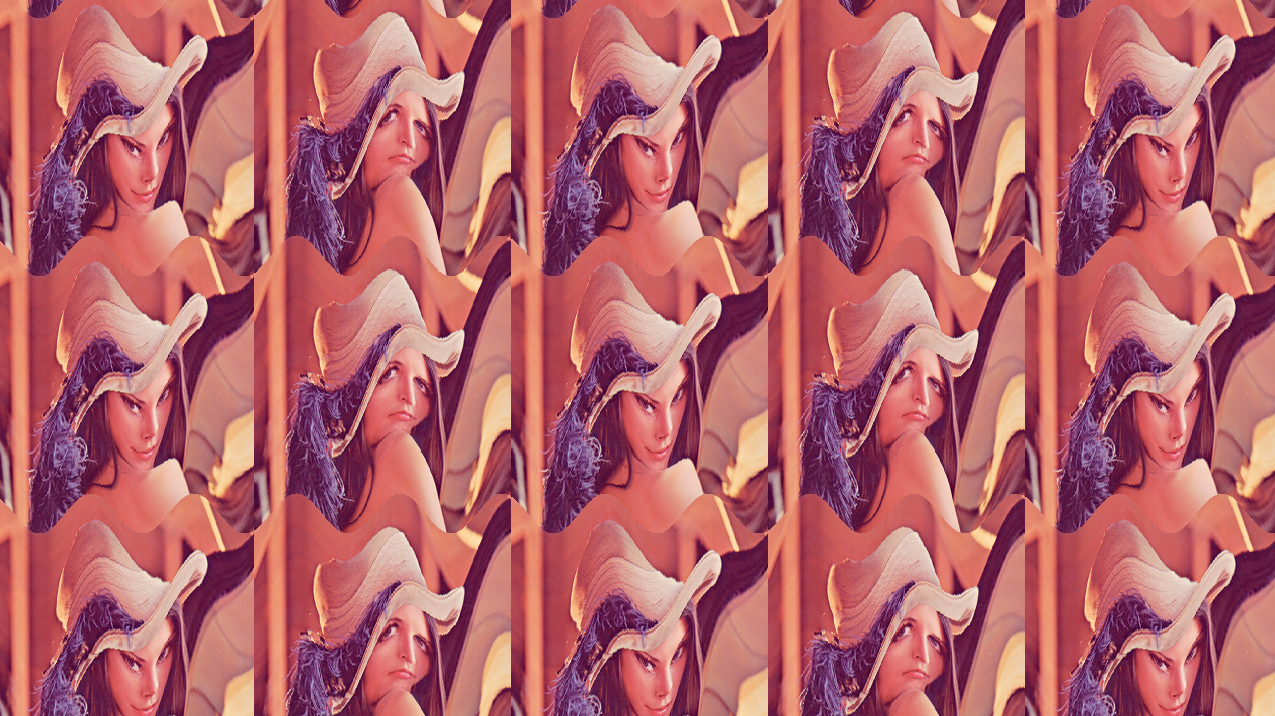
\includegraphics[width=7.5cm]{archivos/deformation2}
		\caption{Onda transversal en x}
	\end{subfigure}
\end{figure}
\begin{figure}\ContinuedFloat
	\centering
	\begin{subfigure}[b]{0.48\textwidth}
		\centering
		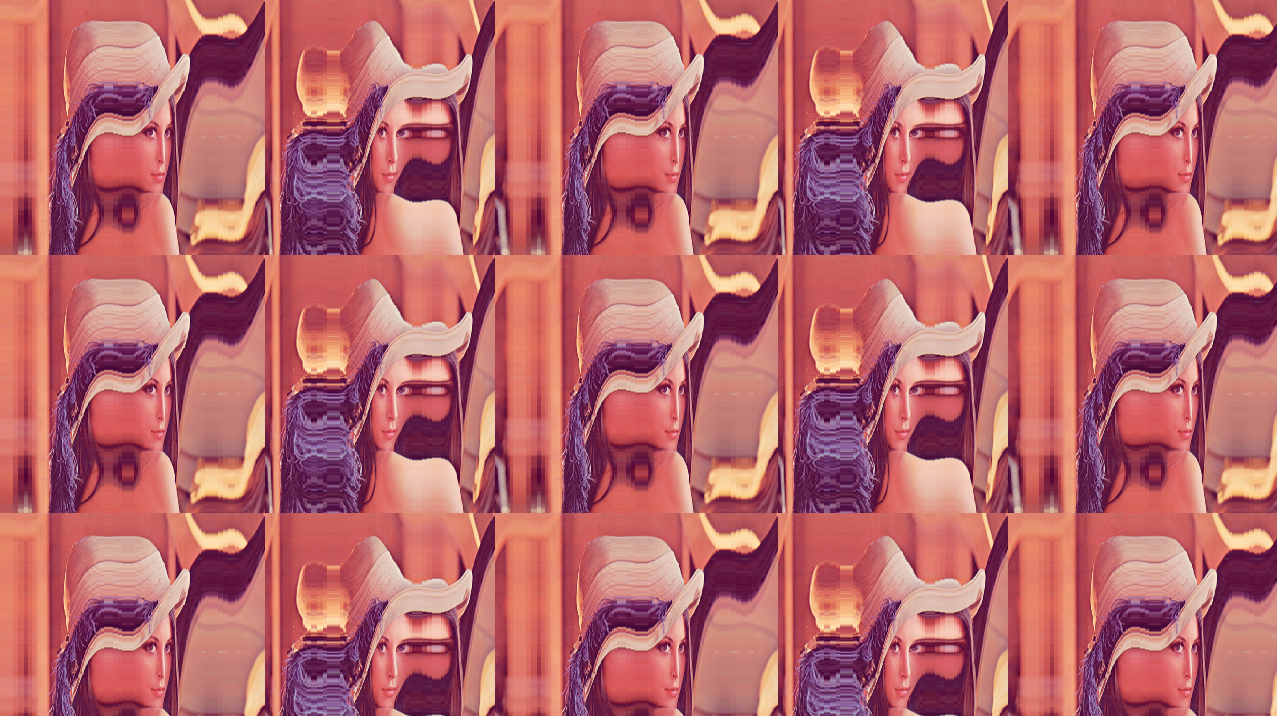
\includegraphics[width=7.5cm]{archivos/deformation3}
		\caption{Onda longitudinal en x}
	\end{subfigure}
	\begin{subfigure}[b]{0.48\textwidth}
		\centering
		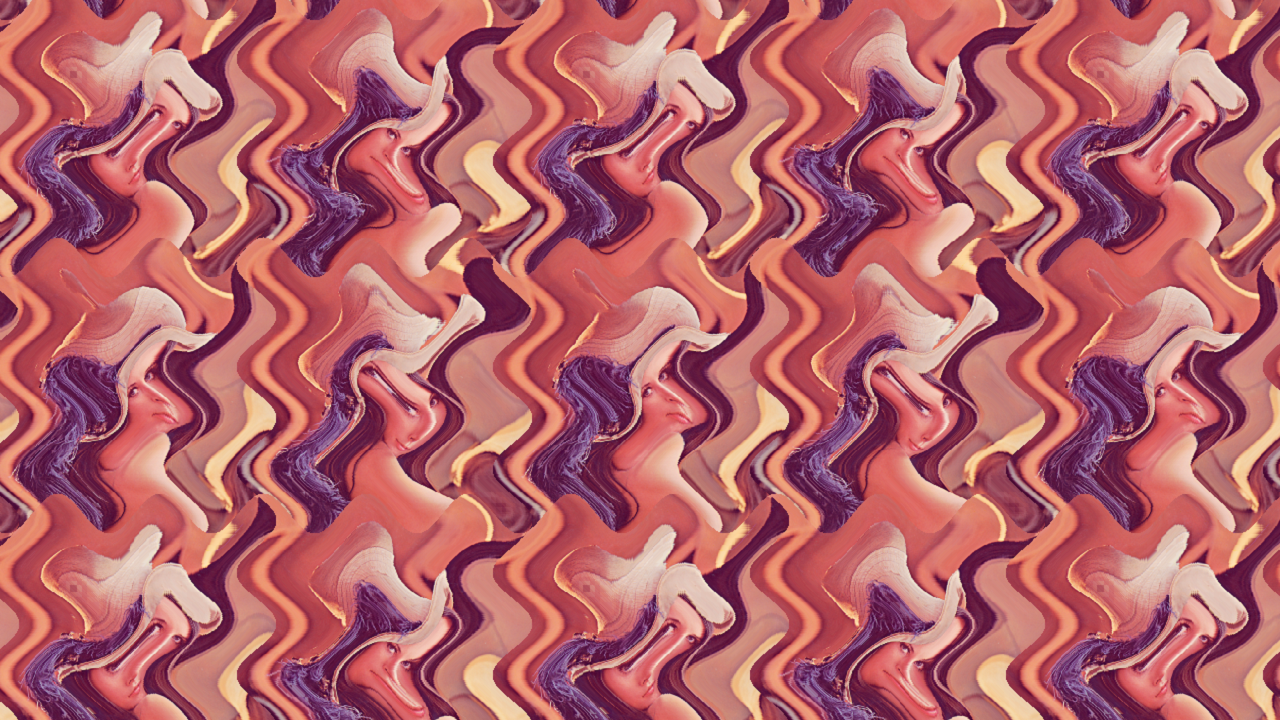
\includegraphics[width=7.5cm]{archivos/deformation4}
		\caption{Transversal en x e y}
	\end{subfigure}
\end{figure}
\begin{figure}\ContinuedFloat
	\centering
	\begin{subfigure}[b]{0.48\textwidth}
		\centering
		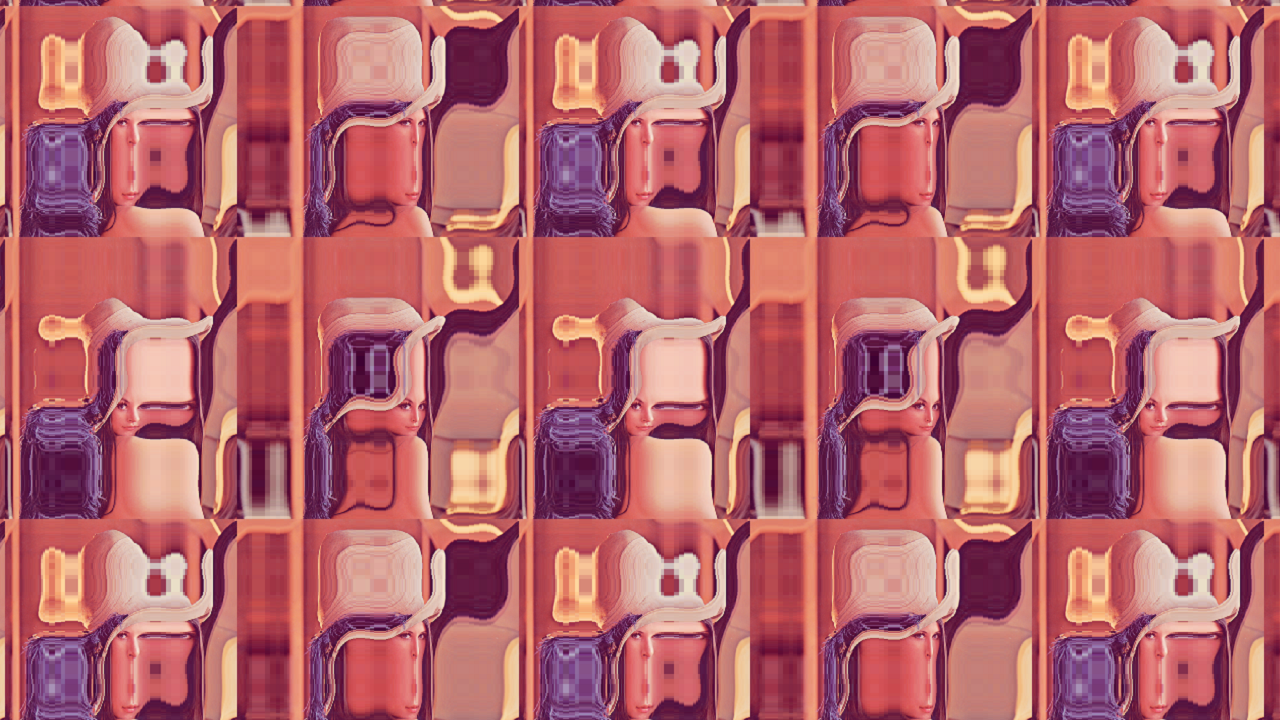
\includegraphics[width=7.5cm]{archivos/deformation5}
		\caption{Mosaico (longitudinal en x e y)}
	\end{subfigure}
	\begin{subfigure}[b]{0.48\textwidth}
		\centering
		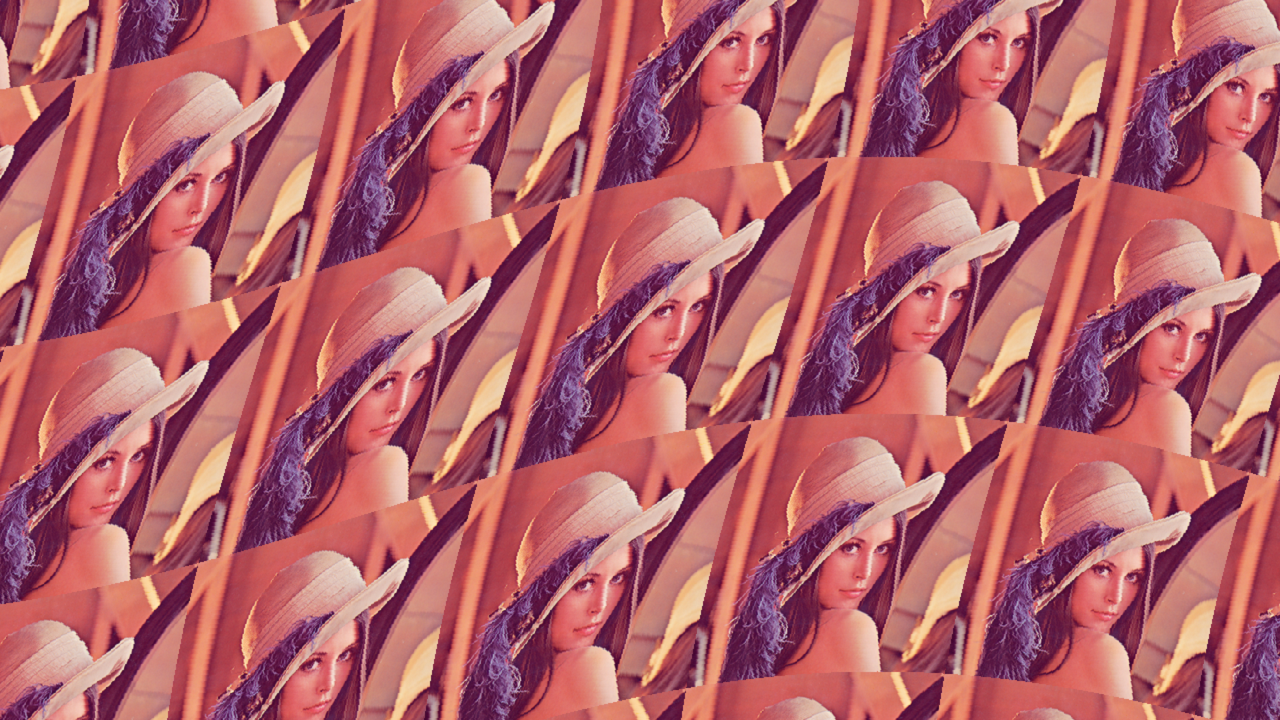
\includegraphics[width=7.5cm]{archivos/deformation6}
		\caption{Efecto de bandera}
	\end{subfigure}
	\caption{Distintos efectos de deformación a partir de ondas}
	\label{fig:alldeformations}
\end{figure}

\section{Plasma}

\subsection{Investigación inicial}

El efecto de plasma es otro de los grandes clásicos de la \emph{demoscene}, como el que podemos ver en la figura [\ref{fig:plasma}]. Este efecto existe bien documentado y podemos encontrar múltiples explicaciones y formas de implementarlo.\\

Un tutorial en detalle, muy bien explicado y documentado es el que podemos encontrar en la página de \textbf{Lode's Computer Graphics Tutorial}\footnote{\url{https://lodev.org/cgtutor/plasma.html}}. Este efecto es tan popular que cuenta incluso con su propia página de Wikipedia\footnote{\url{https://en.wikipedia.org/wiki/Plasma_effect}} e incluso en Rosetta Code\footnote{\url{https://rosettacode.org/wiki/Plasma_effect}} podemos encontrar el código para este efecto implementado en más de 20 lenguajes de programación distintos. También podemos encontrar el código para implementar el efecto de Plasma por GPU en Bidouille.org\footnote{\url{https://www.bidouille.org/prog/plasma}}.\\

Como podemos ver, este no es para nada un efecto desconocido o poco documentado, si no que más bien tenemos que, ante tanta información y tantas implementaciones posibles, elegir la que más se adecue al ámbito de este proyecto.

\subsection{Planteamiento formal}

Existen dos principales acercamientos a la implementación del efecto de plasma: combinación de ondas o generación de ruido.\\

Ambos acercamientos son válidos, e incluso se pueden combinar para producir resultados intermedios. El acercamiento por combinación de ondas se basa en la suma o superposición de distintas funciones de onda, con distintas frecuencias, longitudes de onda y amplitudes, asignando color en función del resultado de la combinación. El acercamiento por generación de ruido se basa, por otro lado, en la generación de un ruido que tenga coherencia local, como por ejemplo el ruido Perlin\footnote{\url{https://en.wikipedia.org/wiki/Perlin_noise}}.\\

Los resultados de generación de ruido mediante Perlin u otros algoritmos de generación de ruido (fractal, simplex...), no obstante, suelen dar resultados más similares a nubes o turbulencias que a plasma, y suelen requerir de niveles bajos de detalle (pocas iteraciones, si se trata de un algoritmo iterativo) o de suavizados posteriores (calculando valores medios o con efectos de desenfoque) para ser suficientemente convincentes. Además de esto, a la hora de animarlos, el movimiento no resulta tan natural como en el uso de ondas, dado que aunque el ruido tenga coherencia local, sigue existiendo un factor de aleatoriedad que puede romper la coherencia del movimiento.\\

Es por ello que se opta por implementar un efecto de plasma mediante la combinación de ondas. Estos serán los pasos a seguir:

\begin{itemize}
	\item Hallar una combinación de ondas que produzca el efecto deseado
	\item Aplicar un degradado de color dado el resultado de la combinación
\end{itemize}

\subsection{Implementación}

En el código [\ref{cod:multiwave}] se muestra una versión simplificada del código para generar ondas, de modo que sea más fácil de leer (dado que el código real emplea tablas precalculadas y guarda cada operación que se repite más de una vez en variables temporales).\\

\begin{lstlisting}[style=C-color, caption={Combinación de distintas ondas}, label=cod:multiwave, escapechar=|]
value += sin((j * i) / (j + i + 1) * scale + accumulatedTime * 191);|\label{line:plasma1}|
value += sin(((width - i) * j) / ((width - i) + j + 1)* scale + accumulatedTime * 157);|\label{line:plasma2}|
value += sin((i * (height - j)) / (i + (height - j) + 1) * scale + accumulatedTime * 113);|\label{line:plasma3}|
value += sin(((width - i) * (height - j)) / ((width - i) + (height - j) + 1) * scale + accumulatedTime * 67);|\label{line:plasma4}|
\end{lstlisting}

Podemos comparar este código con el resultado de la figura [\ref{fig:allwaves}], donde se muestra el resultado que genera cada línea de código, la onda en que resulta de forma separada.\\

\begin{figure}[h]
	\centering
	\begin{subfigure}[b]{0.45\textwidth}
		\centering
		
\includegraphics[width=6cm]{archivos/plasma1}
		\caption{Línea [\ref{line:plasma1}]}
	\end{subfigure}
	\begin{subfigure}[b]{0.45\textwidth}
		\centering
		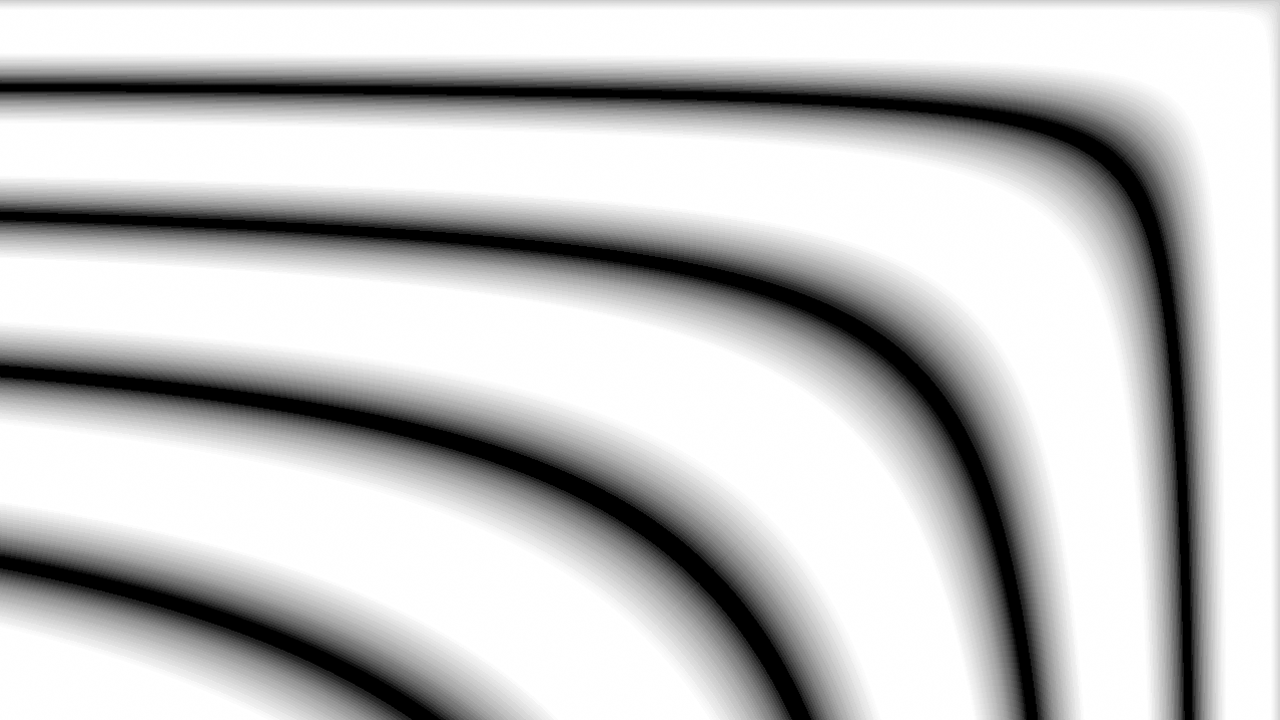
\includegraphics[width=6cm]{archivos/plasma2}
		\caption{Línea [\ref{line:plasma2}]}
	\end{subfigure}
	\begin{subfigure}[b]{0.45\textwidth}
		\centering
		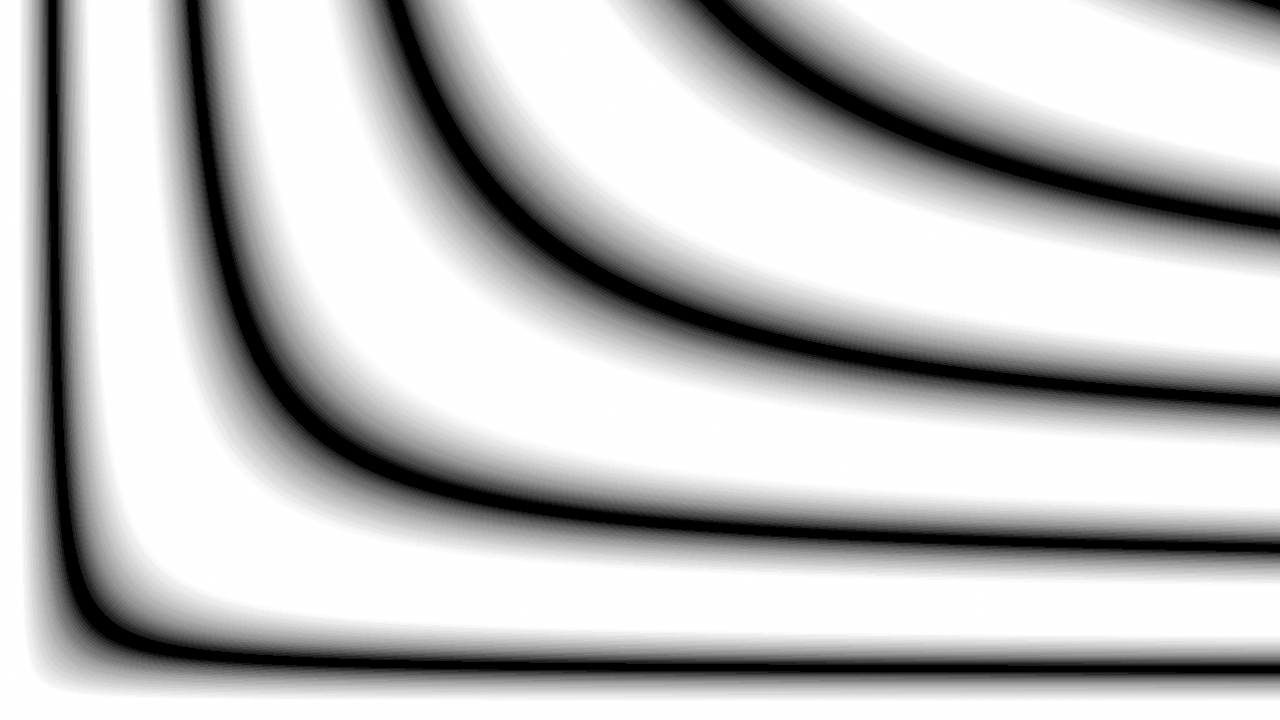
\includegraphics[width=6cm]{archivos/plasma4}
		\caption{Línea [\ref{line:plasma3}]}
	\end{subfigure}
	\begin{subfigure}[b]{0.45\textwidth}
		\centering
		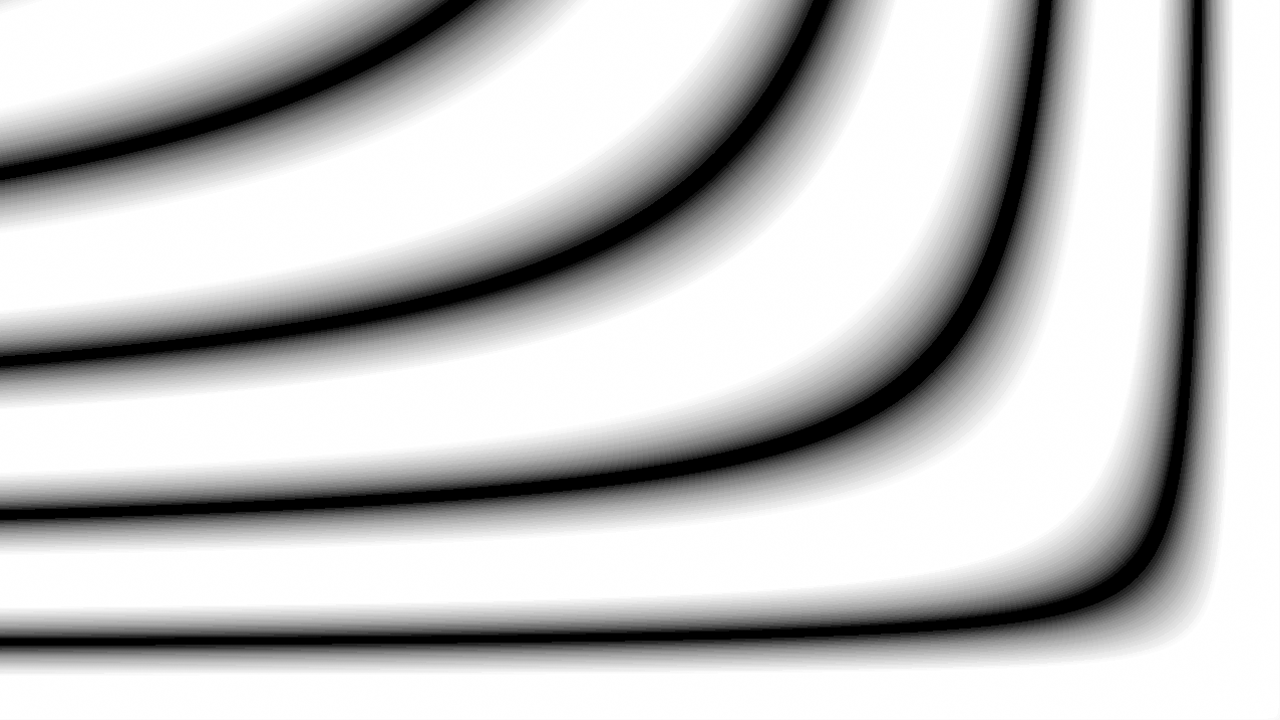
\includegraphics[width=6cm]{archivos/plasma3}
		\caption{Línea [\ref{line:plasma4}]}
	\end{subfigure}
	\caption{Cada una de las ondas que son sumadas (con su correspondencia a línea de código)}
	\label{fig:allwaves}
\end{figure}

Si nos fijamos en el código y en las imágenes, podemos ver que todo lo que hacemos es crear cuatro ondas, yendo cada una hacia una de las esquinas de la pantalla y que están desfasadas entre ellas. Los números elegidos para la fase no son aleatorios, pues todos ellos son números primos. Esto es importante, pues si la fase de alguna onda es múltiplo de otra, se pueden producir formas forzadas o bucles que rompan con la sensación de aleatoriedad y continuidad, dado que su desfase es proporcional. Es por ello que el mejor modo de asegurar que no se produzcan estos \emph{acoples} entre las ondas es multiplicando la fase por números primos, de modo que las fases de las ondas no tengan múltiplos comunes y por tanto no puedan acoplarse o dar sensación de periodicidad.\\  

Una vez hemos sumado nuestras ondas, dividimos entre 4 para normalizar el resultado (entre -1 y 1) y a continuación convertimos este intervalo en un valor entero que oscile entre 0 y 255. De este modo obtenemos un índice con el que acceder a un color específico dentro del degradado de colores que hayamos definido previamente.\\

El resultado de esta combinación de ondas resulta en un efecto bastante convincente, como podemos ver en la figura [\ref{fig:whiteplasma}].\\

\begin{figure}[h]
	\centering
	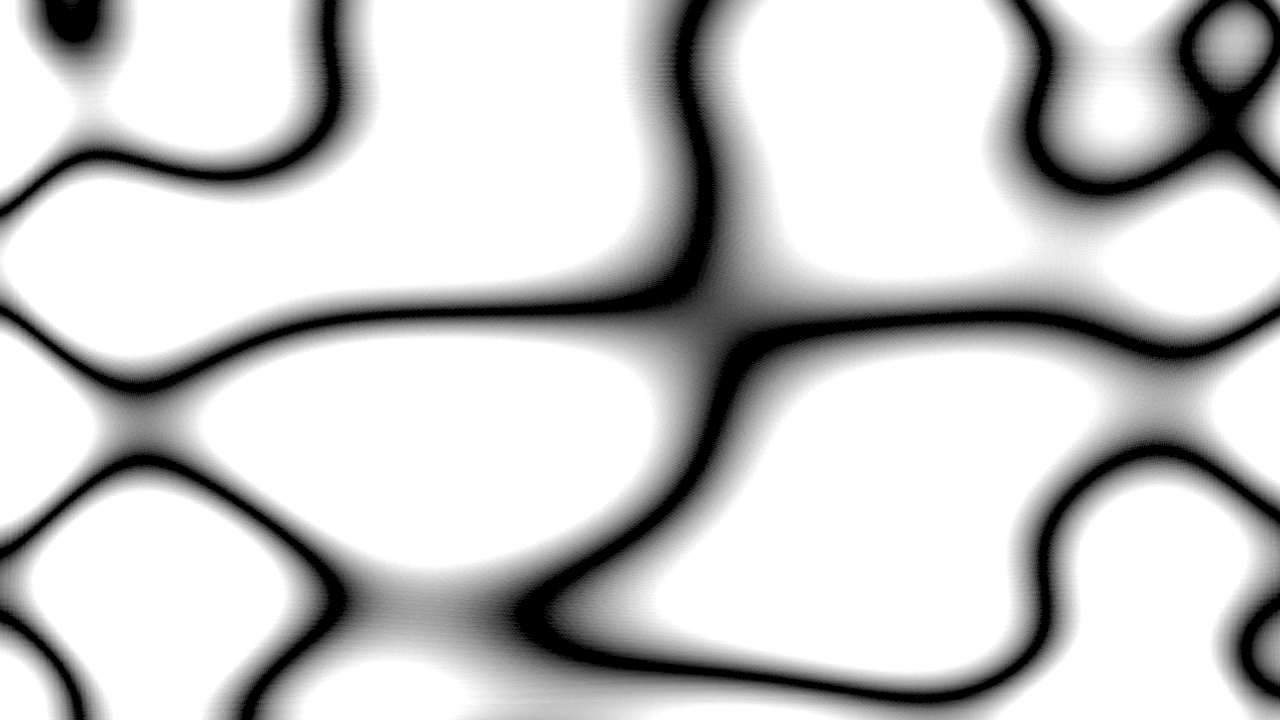
\includegraphics[width=8cm]{archivos/whiteplasma}
	\caption{Efecto de plasma}
	\label{fig:whiteplasma}
\end{figure}

Ahora tan sólo nos queda añadir la capacidad de cambiar de degradado de color, como hemos hecho ya en otros efectos, para conseguir así un resultado más convincente o visualmente impactante.

\subsection{Resultado}

\begin{figure}[h]
	\centering
	\begin{subfigure}[b]{0.48\textwidth}
		\centering
		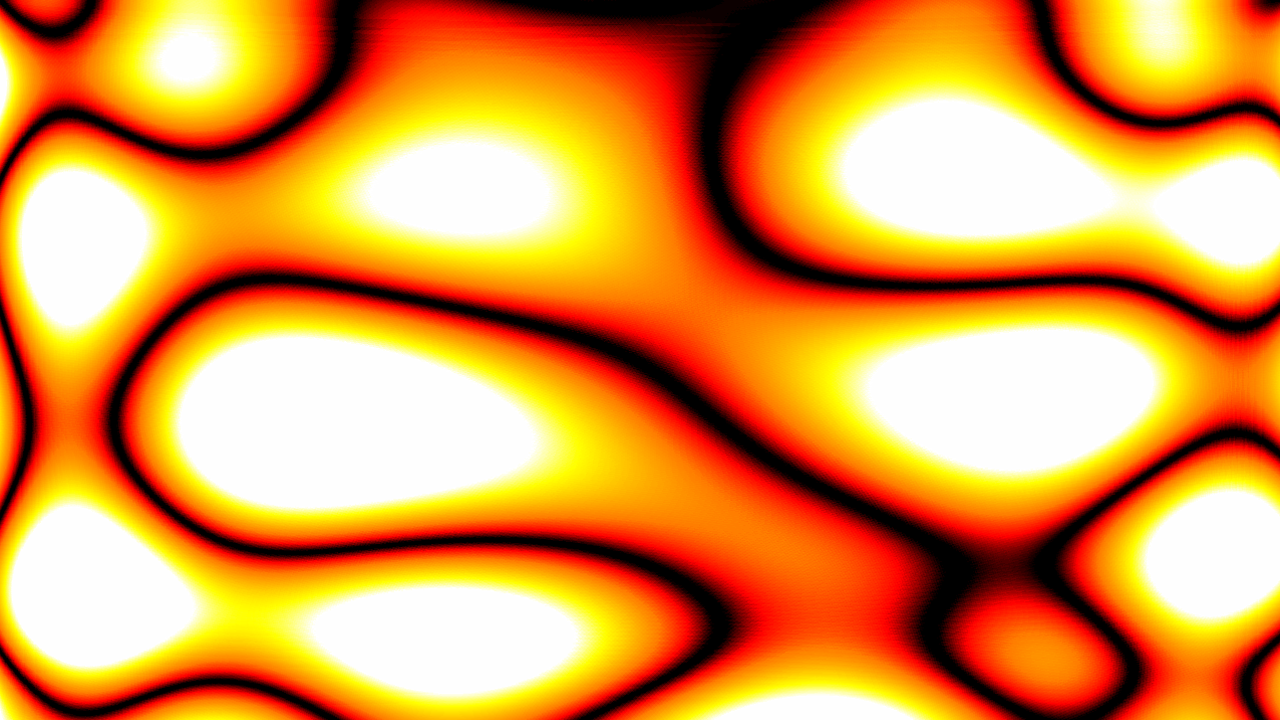
\includegraphics[width=7.5cm]{archivos/redplasma}
		\caption{Efecto lámpara de lava}
	\end{subfigure}
	\begin{subfigure}[b]{0.48\textwidth}
		\centering
		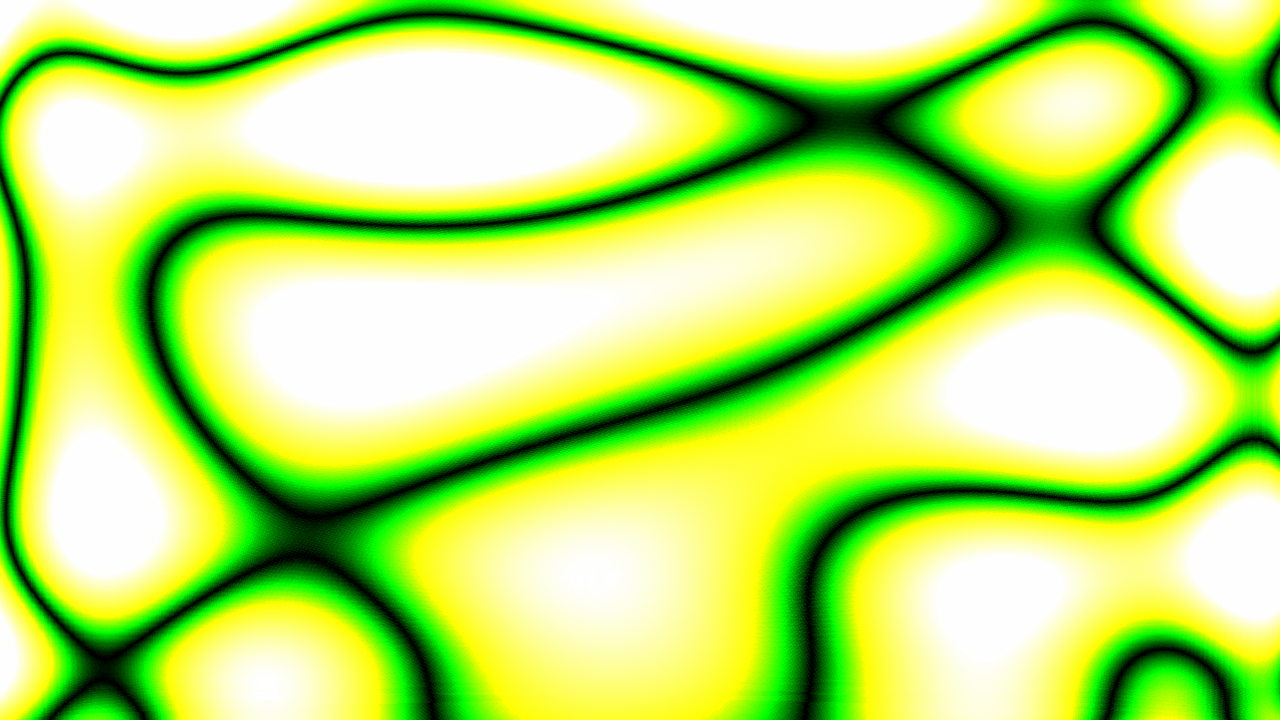
\includegraphics[width=7.5cm]{archivos/greenplasma}
		\caption{Efecto eléctrico}
	\end{subfigure}
\end{figure}

\section{Planos infinitos}

\subsection{Investigación inicial}

El efecto de planos infinitos es muy conocido en la \emph{demoscene}, pero es especialmente popular y conocido en el mundo del videojuego, donde fue popularizado por Nintendo como el famoso Modo 7 \footnote{\url{https://en.wikipedia.org/wiki/Mode_7}} que incluía la SNES. Este era un modo gráfico de esta consola que permitía realizar transformaciones afines, mediante las que se lograba el efecto de planos infinitos.\\

Este efecto básicamente consistía el uso de una textura bidimensional que se transformaba para dar efecto de profundidad o tridimensionalidad, como podemos ver en la figura [\ref{fig:mode7}].\\

\begin{figure}[h]
	\centering
	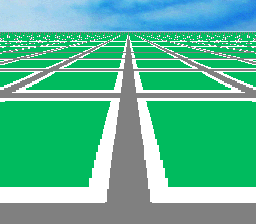
\includegraphics[width=8cm]{archivos/mode7}
	\caption{Modo 7 (efecto de planos infinitos) en la SNES - Fuente: \href{https://en.wikipedia.org/wiki/Mode_7\#/media/File:Mode_7_Test-0000.png}{Wikipedia (por Anomie)}}
	\label{fig:mode7}
\end{figure}

Gracias a este efecto fueron posibles juegos como el primer \emph{Mario Kart}\footnote{\url{https://en.wikipedia.org/wiki/Super_Mario_Kart}}, donde la pista o el circuito no eran más que una textura 2D de grandes dimensiones transformada, para que pareciera un plano o un circuito 3D.\\

Este efecto está muy bien documentado y se puede encontrar su explicación formal tanto en Wikipedia como numerosos tutoriales que ofrecen distintos acercamientos, como este tutorial de \emph{One Lone Coder}\footnote{\url{https://www.youtube.com/watch?v=ybLZyY655iY&t=646s}} en que ofrece una explicación formal y da su propio planteamiento para implementar este modo o este otro tutorial en Coranac.com\footnote{\url{https://www.coranac.com/tonc/text/mode7.htm}} dónde se nos ofrecen tres implementaciones distintas, con distintos acercamientos, y se hace una reflexión sobre los resultados obtenidos.

\subsection{Planteamiento formal}

El efecto de planos infinitos está muy bien documentado, bajo distintos acercamientos, uno de los cuales es el Modo 7, aunque también existen otras formas de causar un efecto similar.\\

Siguiendo el espíritu de este trabajo, intentaremos implementar el efecto de planos infinitos sin usar código de referencia, simplemente usando el material visual disponible para intentar deducir cómo podríamos implementar este efecto. En la figura [\ref{fig:planes}], de creación propia, vemos un posible acercamiento a este efecto, que es el que seguiremos e intentaremos implementar.\\

\begin{figure}[h]
	\centering
	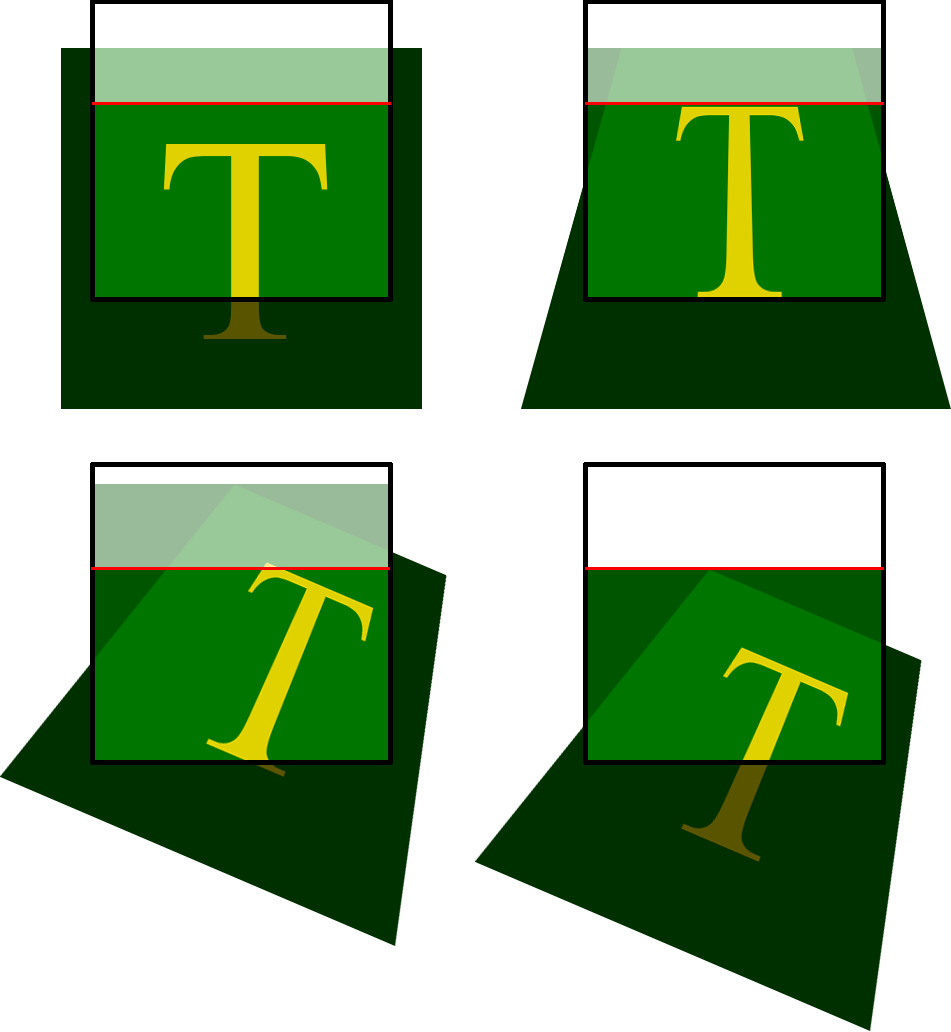
\includegraphics[width=12cm]{archivos/planes}
	\caption{Nuestro acercamiento a los planos infinitos}
	\label{fig:planes}
\end{figure}

En esta figura [\ref{fig:planes}], el cuadro negro representa la pantalla o la parte visible de la textura, la línea roja representa la línea del horizonte, punto a partir del cual no se muestra nuestra textura en pantalla.\\

Para facilitar la visualización del contenido, la parte de la textura fuera de pantalla se ha oscurecido y la parte de la textura en pantalla pero tras la linea del horizonte se ha aclarado, de modo que la porción visible destaque. Además, se ha rellanado el espacio en de pantalla adyacente a nuestra textura con un verde más oscuro, para completar la imagen y facilitar su visualización.\\

Como vemos, partimos de una textura bidimensional, plana. A continuación, estiramos la textura en su parte baja y la apretamos en la parte alta. Dicho de un mejor modo: hacemos nuestra textura depender de la altura, de modo que a mayor altura, más se estreche y viceversa. Ya solo con esto, nuestra imagen gana sensación de profundidad y tridimensionalidad. Pero además, queremos ser capaces de moverla. Para ello, una vez que nuestra textura ha sido convenientemente deformada, rotamos la imagen usando la fórmula mostrada en la figura [\ref{fig:transform}].\\

Una vez que nuestra textura ha sido deformada y rotada como queremos, podemos desplazarla, de modo que así, es pantalla, dará sensación de movimiento y avance. Realmente, todo lo que hacemos es aplicarle las transformaciones 2D que ya vimos con el RotoZoom pero con un contexto y un fin distintos.

\subsection{Implementación}

\begin{lstlisting}[style=C-color, caption={Código para generar un efecto básico de planos infinitos, con escalado, rotación y translación}, label=cod:infiniteplanes, escapechar=|]
for (int j = 0, nh = height / 2; j < nh; j++)
{
    for (int i = -width / 2, nw = width / 2; i < nw; i++)
    {
        Point2D projectedPoint(i / (float)j, fieldOfView / (float)j);|\label{line:planesproject}|
        projectedPoint *= textureScale;|\label{line:planesscale}|
        
        Point2D rotatedPoint(projectedPoint.X * cosine - projectedPoint.Y * sine,
                                projectedPoint.X * sine + projectedPoint.Y * cosine);
                             
        Pixel colour = texture[Fast::Abs((int(rotatedPoint.Y + cameraPosition.Y) % texHeight) * texWidth +
                                            int(rotatedPoint.X + cameraPosition.X) % texWidth)];
                                         
        pixels[(j + nh) * width + (i + nw)] = colour;|\label{line:planesaccess}|
    }
}
\end{lstlisting}

Como podemos ver en el código, recorremos media pantalla en altura, desde 0 hasta la mitad de la pantalla, y desde \(-x \div 2\) hasta \(+x \div 2\), recorriendo así toda la anchura de la pantalla. Esta decisión no es aleatoria, pues como vemos más adelante, en la línea [\ref{line:planesaccess}] sumamos la mitad de la altura y la anchura, desplazando las coordenadas \emph{i} y \emph{j}. Hacemos esto por conveniencia, pues nos facilita los cálculos, ya que para transformar nuestra textura lo hacemos con respecto al origen de la pantalla (el \emph{(0, 0)} equivale a la esquina superior izquierda) y luego desplazamos el resultado obtenido, como podemos ver en la figura [\ref{fig:desplazamiento}].\\

\begin{figure}[h]
	\centering
	
\includegraphics[width=8cm]{archivos/desplazamiento}
	\caption{Posición relativa de la textura antes y después de ser transformada}
	\label{fig:desplazamiento}
\end{figure}

Esto es importante también porque además de facilitar los cálculos, operar con la coordenada horizontal de la textura centrada en el origen es el equivalente a situar nuestra "cámara", es decir, nuestro punto de vista en el origen. Si hacemos los cálculos de este modo, el punto de fuga del resultado obtenido se situará en el centro de la pantalla (ya que calculamos con respecto al origen -punto de fuga- y luego desplazamos el resultado). Esto da un resultado mucho más realista, pues en nuestra visión el punto de fuga siempre tiende hacia el centro. Podemos ver una demostración visual en la figura [\ref{fig:planes1}].\\

\begin{figure}[h]
	\centering
	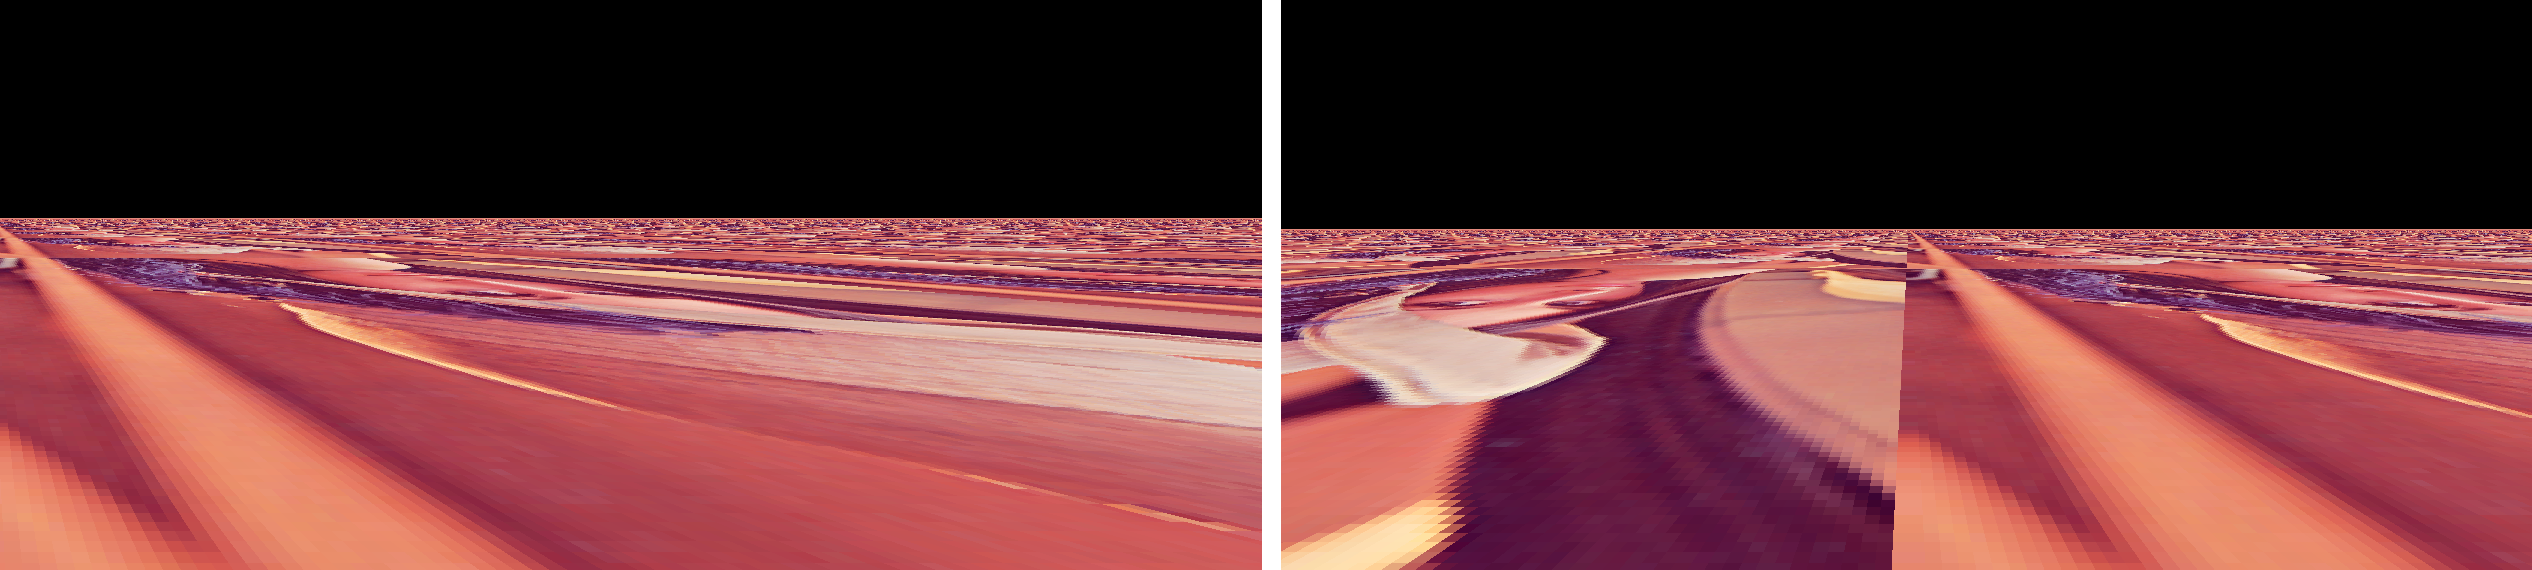
\includegraphics[width=14cm]{archivos/planes1}
	\caption{A la izquierda el punto de fuga está en el 0 de las coordenadas horizontales, a la derecha está en el centro}
	\label{fig:planes1}
\end{figure}

En la figura [\ref{fig:planes1}], la imagen de la izquierda se obtiene iterando de 0 a la anchura de la pantalla en la coordenada horizontal. Como el origen está al inicio de la pantalla, todo se siente desplazado hacia la izquierda, de forma poco natural. En la imagen de la derecha, iteramos desde \(-anchura \div 2\) hasta  \(+anchura \div 2\) y luego desplazamos el resultado en \(anchura \div 2\), situando de este modo el punto de fuga en el centro del imagen, tal y como se da en nuestra visión, en el mundo real.\\

Dentro del bucle, empezamos por la primera transformación (equivalente a estirar la textura en la parte inferior y estrechar en la superior, como veíamos en la figura [\ref{fig:planes}]). Para obtener este efecto, basta con dividir basándonos en la altura, como podemos ver en la línea [\ref{line:planesproject}]. A mayor sea la altura (recordemos que el eje Y está invertido en una pantalla, por lo que mayor altura es más hacia abajo), menor será nuestra el índice con el que accederemos a nuestra textura. Esto causa que a mayor sea la altura, menor es la distancia entre los accesos a la textura y por tanto la textura tiene una apariencia más grande. Es por esto que a menos altura (más arriba), la textura se percibirá más comprimida y a mayor altura (más abajo) los accesos a memoria serán más contiguos y por tanto la imagen resultante se percibirá más grande. Podemos ver este efecto claramente en la figura [\ref{fig:planes1}].\\

Además, como podemos ver en la línea [\ref{line:planesproject}], nuestra variable horizontal depende de la vertical (\emph{i} depende de \emph{j}), y para la coordenada vertical del punto que creamos, usamos una variable definida por el usuario y que también se ve afectada por la altura (que equivale a la distancia desde el observador, es decir, más arriba en pantalla implica menor altura y más distancia desde el observador si en lugar de una textura plana se tratase de un espacio tridimensional real). A esta variable la llamamos \emph{field of view}, o campo de visión, y su modificación modifica el ángulo o la amplitud con la que vemos en pantalla, como podemos ver en la figura [\ref{fig:planes2}].

\begin{figure}[h]
	\centering
	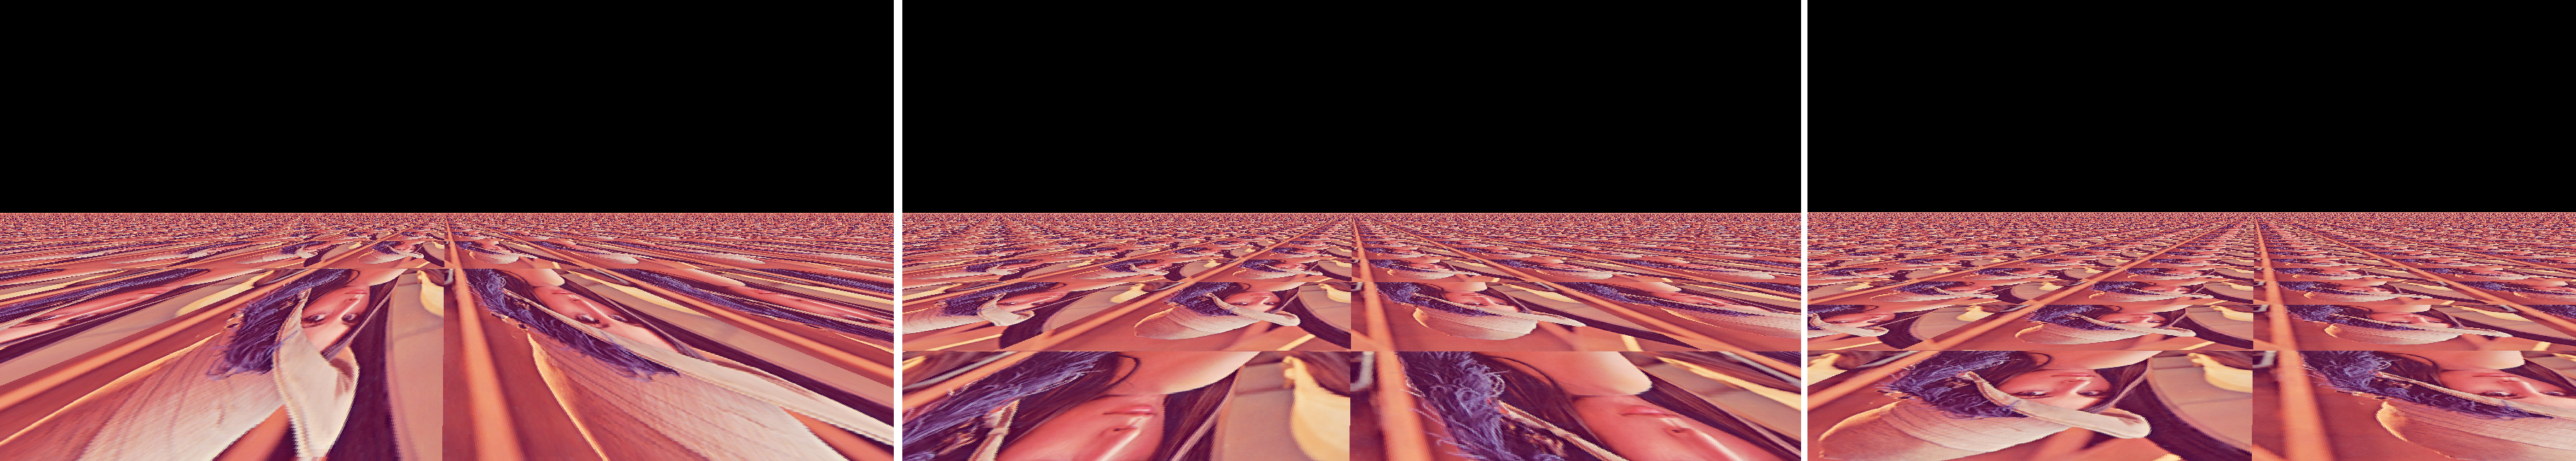
\includegraphics[width=14cm]{archivos/planes2}
	\caption{De izquierda a derecha, de mayor a menor campo de visión}
	\label{fig:planes2}
\end{figure}

A continuación, escalamos nuestra textura por un factor, como podemos ver en la línea [\ref{line:planesscale}]. Esto variará el tamaño de nuestra textura en pantalla, y por tanto, también el número de repeticiones de la misma. A menor sea la escala, menor será la textura y más repeticiones se darán de la misma para llenar la pantalla.\\

Tras el escalado, rotamos nuestra textura en función de un ángulo que se corresponderá con el giro de cámara, aplicando la fórmula matemática ya vista en la figura [\ref{fig:transform}], y a continuación sumamos el desplazamiento, que se corresponderá con la posición de la cámara en la escena. Tras ello, aplicamos el módulo para asegurarnos que si se sobrepasan los límites de nuestra textura, se produzca un acceso cíclico a la misma, y no se den errores de acceso. Nos aseguramos además de que el resultado obtenido sea positivo (calculando el valor absoluto) para evitar así accesos negativos que puedan hacer fallar nuestra aplicación. Una vez hemos calculado las coordenadas de la textura que se corresponden con las coordenadas en pantalla, y una vez que hemos obtenido el color al que se asocian nuestras coordenadas de textura, asignamos el color.\\

Con esto, obtenemos una escena que produce la sensación de planos infinitos y por la que nos podemos mover como si se tratase de un videojuego en primera persona (pues podemos modificar la rotación, escala y traslación, que en nuestra escena es el equivalente a mover la cámara).\\

Podemos ver además que para esta demo hemos creado una estructura a la que hemos denomidado \lstinline{Pixel2D}\{. Esta es una estructura sencilla que simplemente nos permite almacenar dos coordenadas en coma flotante con precisión simple (\emph{x} e \emph{y}) y nos da facilidades para operar con las mismas (suma y resta de puntos, multiplicación por un escalar...).

\subsection{Refinamiento}

\begin{itemize}
	\item \textbf{Fundido a negro}: actualmente, la línea del horizonte pasa directamente de tener color a un horizonte negro. Este cambio puede resultado algo brusco. Si creamos una variable de opacidad que dependa de la altura, de modo que a menor sea la altura menos sea la opacidad (es decir, a más lejos esté la cámara del observador, más oscuro se vea) conseguiremos un efecto mucho menos brusco y mucho más ambiental. 
	\item \textbf{Relieve}: un pequeño añadido que me pareció que podría ser curioso de implementar consiste en una falsa sensación de relieve que dependa del brillo del color. Para hacer esto, lo que hacemos es desplazar el dibujado de nuestra textura en un factor variable que dependa del brillo del color que aplicamos, de modo que los colores más oscuros se pinten más abajo y los colores más claros más arriba en pantalla, dando así una cierta sensación de relieve o terreno, sumando a la sensación de tridimensionalidad. Como podemos ver en el código [\ref{cod:displacement}], empezamos por calcular la percepción del brillo en base al color, tal y como es percibido por el ojo humano\footnote{\url{https://en.wikipedia.org/wiki/Relative_luminance}} y a continuación multiplicamos por 0.004 (equivalente de dividir por 256) para normalizar el resultado. Tras ello, calculamos el desplazamiento de la textura en función del nivel de desplazamiento (decidido por el usuario), el brillo relativo del color y la distancia al observador. Aplicamos este desplazamiento al asignar el color en pantalla.
\end{itemize}

\begin{lstlisting}[style=C-color, caption={Código para calcular el desplamiento de la textura}, label=cod:displacement]
float colourBrightness = ((colour.R * 0.3) + (colour.G * 0.59) + (colour.B * 0.11)) * 0.004f; // * 1 / 256
int textureDesplacement = (bumpLevel * colourBrightness) * distanceFactor;
pixels[(j - textureDesplacement + nh) * width + (i + nw)] = colour;
\end{lstlisting}

\subsection{Resultado}

\begin{figure}[h]
	\centering
	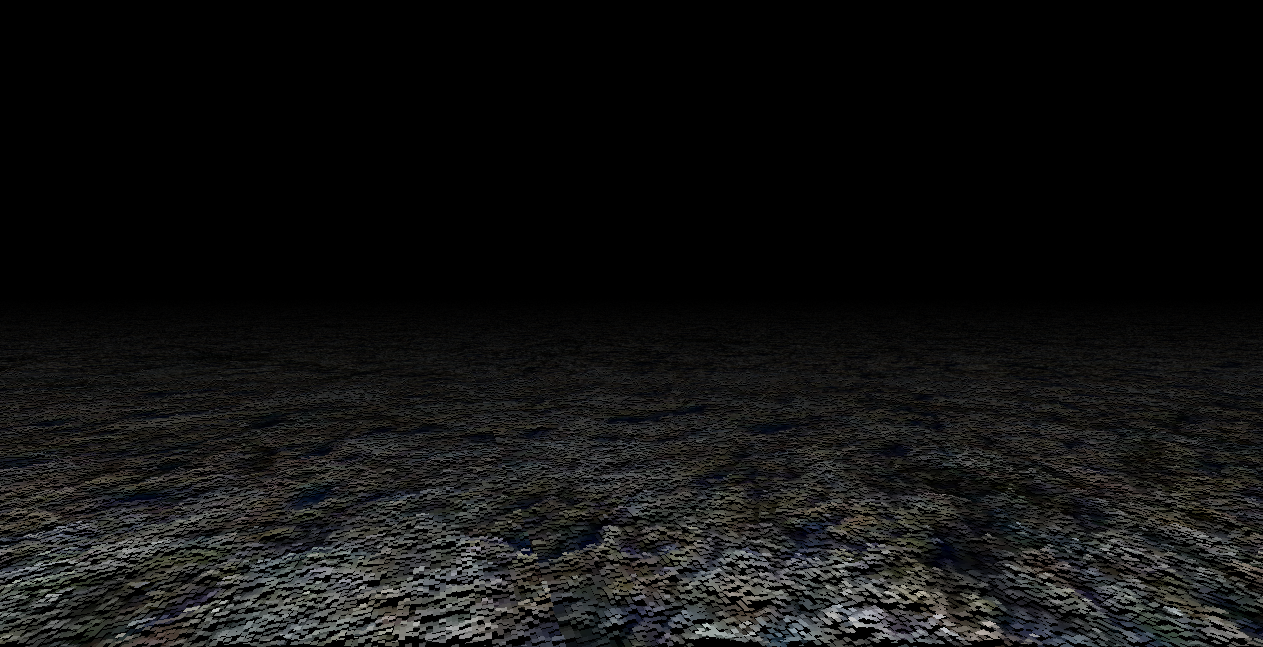
\includegraphics[width=12cm]{archivos/planes3}
	\caption{Resultado final, con efectos de niebla y relieve aplicados}
	\label{fig:planes3}
\end{figure}

\section{Geometría}


\subsection{Investigación inicial}

De cara al efecto de geometría, lo tenía claro: quería realizarlo desde 0, basándome puramente en el planteamiento matemático, y tratando de desarrollar un solución lo más simple pero efectiva posible.\\

Para poder realizar un efecto completo es necesario un motor gráfico que nos permita gestionar cámaras, múltiples instancias de objetos, orden de dibujado y optimizaciones para no dibujar objetos fuera de pantalla, no dibujar objetos que son tapados por otros objetos, etc...\\

Implementar todas estas características parecía a todas luces inviable, pues desarrollar un motor gráfico complejo conlleva su propio trabajo e investigación, y se sale del ámbito de este proyecto. Es por ello que se optó por un planteamiento basado puramente en la matemática y abogando por la simplicidad.\\

No obstante, y a modo de nota, dejo apuntados dos grandes canales de referencia para la implementación de un motor gráfico completo partiendo desde cero, siendo uno el ya varias veces mencionado en este trabajo \emph{One Lone Coder}\footnote{\url{https://www.youtube.com/watch?v=ih20l3pJoeU}} y otro la lista de reproducción de \emph{Chili Tomato Noodle}\footnote{\url{https://www.youtube.com/watch?v=uehGqieEbus&list=PLqCJpWy5Fohe8ucwhksiv9hTF5sfid8lA}}.

\subsection{Planteamiento formal}

Como ya hemos dicho, no vamos a implementar un motor gráfico completo, si no que vamos a tratar de implementar el motor más sencillo posible a partir de pura deducción matemática. Es por ello que vamos a sacrificar cierta flexibilidad, a cambio de una mayor sencillez:

\begin{itemize}
	\item \textbf{Evitaremos el uso de matrices}: los motores gráficos actuales usan matrices 4x4 para el cálculo de coordenadas. Esto es muy útil pues permite un sistema de coordenadas y transformaciones homogéneas\footnote{\url{https://en.wikipedia.org/wiki/Homogeneous_coordinates}}, lo que significa que el estado de transformación de cualquier objeto (escala, rotación y traslación) puede ser guardado y/o acumulado en una sola matriz, haciendo así que aplicar transformaciones geométricas sea un proceso fácilmente automatizable y mantenible. Esto viene al coste, no obstante, de tener que gestionar multiplicaciones de matrices, operación que no es trivial, pues para multiplicar una matriz 4x4 por otra, es necesario multiplicar los 16 elementos que forman una matriz por los 16 de la otra, lo que equivale a 256 multiplicaciones. El uso de matrices aporta flexibilidad, mantenibilidad y un modelo matemático único y sólido, pero lo hace al coste de eficiencia (la multiplicación de matrices no es trivial) y de complejidad (manipular matrices requiere una base matemática sólida).
	\item \textbf{Cámara fija en el origen}: nuestra cámara se mantendrá fija en el origen de las coordenadas y no podremos desplazarla. Normalmente para desplazar la cámara en un motor gráfico convencional, lo que se hace realmente es trasladar el \emph{mundo} con respecto a la cámara, que se mantiene siempre en el origen. Para hacer esto, se suele hallar la matriz inversa\footnote{\url{https://en.wikipedia.org/wiki/Invertible_matrix}} de la transformación de la cámara y multiplicar cada elemento en escena por la misma, para así desplazarlo en función del "movimiento" de la cámara, que se mantiene estática en el origen. Por supuesto, esta operación se puede realizar sin usar matrices, simplemente transformando cada objeto con la transformación inversa que se aplica a la cámara (si la cámara se desplaza hacia la derecha, en lugar de mover la cámara, la mantenemos en el origen y movemos nuestros objetos en escena hacia la izquierda). Sin embargo, esto aporta una complejidad añadida y una cantidad de cálculo extra que no resulta excesivamente práctica de cara al resultado final, que no se verá excesivamente impactado por tener una cámara fija.
	\item \textbf{Orden de dibujado dependiente del orden de los vértices}: usualmente, para evitar que objetos que están "virtualmente al fondo" se dibujen por encima de los que están "más adelante" en pantalla, se utilizan \emph{buffers} de profundidad, también conocidos como \emph{z-buffer}\footnote{\url{https://en.wikipedia.org/wiki/Z-buffering}}. Estos \emph{buffers} funcionan a nivel de píxel, y se aseguran que solo se pinte en pantalla el píxel que más cercano está al observador (si dos objetos, una verde y uno azul, se superponen en un mismo píxel, el color final del píxel dependerá de qué objeto está delante, y no de qué vertice se dibujó primero). No obstante, mantener un \emph{buffer} de profundidad aumenta la complejidad tanto espacial como temporal de la solución, y resulta poco práctico cuando sólo vamos a tener unos pocos objetos sencillos en pantalla.
	\item \textbf{Pintaremos únicamente el \emph{wireframe} de los objetos}: sólo dibujaremos las aristas de los objetos, pero no los dibujaremos como objetos sólidos ni les aplicaremos textura. Esta decisión se toma no tanto por cuestión de complejidad de implementación como por cuestión de eficiencia. En primer lugar, si nuestros objetos son sólidos, entonces se hace mucho más necesario tener un \emph{buffer} de profundidad. Que las aristas de un objecto cualquiera intersecten con si mismas no supone un problema grave, y apenas suele ser perceptible, pero si la parte trasera del cubo se dibuja por encima de la delantera, se producen defectos visuales serios. Pero más allá de esto, dibujar tan sólo las aristas de nuestro objeto implica tener que pintar unos pocos píxeles (se dibujan líneas, únicamente), mientras que hacer nuestros objetos sólidos implica tener que rellenar todo el espacio que ocupa el objeto, teniendo que pintar una gran cantidad de píxeles. Si a esto le sumásemos aplicar una textura al objeto (operación relativamente sencilla, pues consiste en un \emph{mapping} entre la posición en el espacio del objeto y el acceso a la textura, consistiendo en una simple transformación), nos topamos con un coste temporal para nada trivial. La diferencia para dibujar un objeto pasa a ser de pintar unas pocas líneas en cualquier orden a tener que pintar todo el espacio que ocupa el objeto píxel a píxel y asegurar por píxel que se pinta el color de la cara que está más al frente y que esté correctamente \emph{mapeado} a la textura que corresponde al objeto. Recordemos que estamos en CPU, no nos podemos permitir toda esta cantidad de cálculo a altas resoluciones de pantalla. Es por algo, al fin y al cabo, que se crearon la unidades gráficas (GPU) para manejar las operaciones con gráficos (operaciones sencillas a nivel matemático -pues suelen ser sumar, restas, multiplicaciones y divisiones- pero con gran carga computacional -pues hay que realizar miles o millones de ellas por fotograma-).
	\item \textbf{No dejaremos de pintar objetos por estar fuera de pantalla o ser tapados por otros objetos}: técnicas como el \emph{clipping}\footnote{\url{https://en.wikipedia.org/wiki/Clipping_(computer_graphics)}} o el \emph{culling}\footnote{\url{https://en.wikipedia.org/wiki/Back-face_culling}} evitan el pintado de objetos o partes del objeto que están fuera de pantalla o que no son visibles. Estas técnicas de optimización tienen sentido absoluto cuando pintamos una gran cantidad de caras sólidas con texturas, pues el coste de pintar una cara no es para nada trivial, y es mucho menor el coste de calcular qué caras u objetos deben ser pintados que pintarlo todo a fuerza bruta. En nuestro efecto, sin embargo, pintaremos pocos objetos, que rara vez se saldrán de pantalla y que no serán objetos sólidos, por lo que aplicar técnicas de optimización de este estilo sólo aumentará la complejidad del código sin ofrecer ganancias reales.
\end{itemize}

\subsection{Implementación}

Para poder dibujar un objeto tridimensional en una pantalla bidimensional, debemos encontrar un modo de representar el objeto y dibujarlo. Para ello, necesitamos almacenar los puntos que forman nuestro objeto y la relación entre ellos (qué pares de puntos están conectados formando aristas). Además, necesitamos encontrar un modo de proyectar nuestros puntos tridimensionales contra un plano, que se corresponderá a nuestra pantalla, de modo que podamos ver una representación 2D de nuestro objeto tridimensional.\\

En la figura [\ref{fig:projection}] podemos ver un ejemplo de proyección paralela, donde se trazan líneas paralelas desde cada punto del objeto y se calcula su intersección con respecto a un plano bidimesional. Luego, los puntos resultado de la intersección se unen entre sí, siendo las líneas resultantes las aristas proyectadas de nuestro objeto tridimensional. Como veremos más adelante, a nivel de implementación, la proyección paralela es muy sencilla de realizar.\\

\begin{figure}[h]
	\centering
	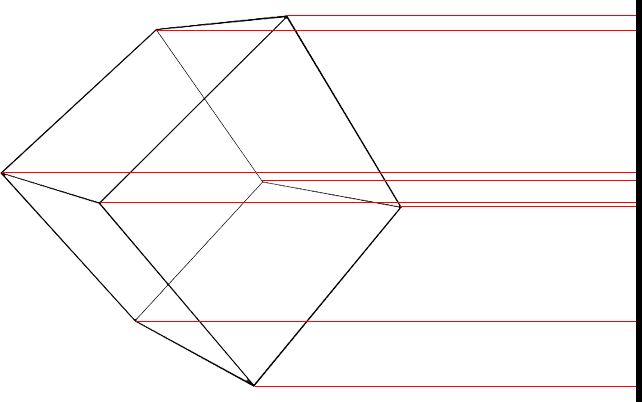
\includegraphics[width=7cm]{archivos/projection}
	\caption{Cubo 3D que se proyecta contra el plano (proyección paralela)}
	\label{fig:projection}
\end{figure}

Así pues, empezamos por crear dos nuevas estructuras, como podemos ver en la figura [\ref{fig:pointandobject}]. Son el punto 3D, muy similar al punto 2D previamente creado, pero con una dimensión extra, y el objeto 3D. Un objeto 3D consiste en una serie de puntos que representan la posición en el espacio 3D de los vértices del objeto a representar y un conjunto de pares de índices. Cada índice referencia la posición de uno de los vértices en la lista de puntos. De este modo, cada par de índices representa una arista de nuestro objeto a dibujar. Adicionalmente se incluye un conjunto de puntos 2D al que llamamos \emph{projectedPoints}. Este vector se corresponde con el vector de vértices, y contiene los puntos tridimensionales una vez que son proyectados contra la pantalla, y por tanto convertidos al espacio 2D.\\

\begin{figure}[h]
	\centering
	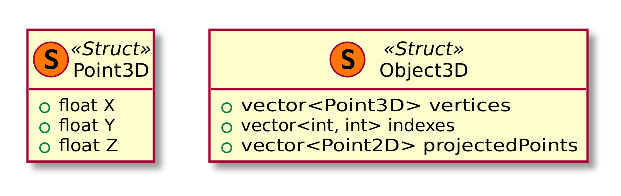
\includegraphics[width=12cm]{archivos/pointandobject}
	\caption{Estructura básica de Point3D y Object3D}
	\label{fig:pointandobject}
\end{figure}

Una vez tenemos un modo de representar nuestros objetos, es necesario hallar una forma de proyectarlos. Como hemos anticipado, la proyección de un objeto con respecto al plano \(z = 0\) es extremadamente sencillo. Este es el plano que tiene su centro en el origen de coordenadas y se extiende infinitamente en \emph{x} e \emph{y}. La intersección de cualquier línea perpendicular a este plano con el mismo será equivalente a un punto de las características \emph{(x, y, 0)}, dado que \emph{z} siempre equivale a 0. Como para hallar nuestra proyección paralela lo que hacemos es hallar el punto de intersección de una recta perpendicular al plano de proyección que pasa por un vértice de nuestro objeto a proyectar, este punto de intersección siempre será del tipo \emph{(x, y, 0)}. O en otras palabras, para obtener nuestro punto proyectado con respecto a \(z = 0\), ¡todo lo que tenemos que hacer es tomar las coordenadas \emph{x} e \emph{y} e  ignorar el valor de \emph{z}!\\

Una vez tenemos una forma de representar un objeto 3D y una forma extremadamente sencilla de proyectarlo, llega el momento de dibujarlo. Como podemos ver en el código [\ref{cod:renderobject}], todo lo que tenemos que hacer es recorrer todos los pares de índices y por cada par, obtener el punto de inicio y final de la arista proyectada. A continuación, dibujamos una línea que vaya de un punto al otro y ¡ya podemos dibujar figuras tridimensionales en pantalla!\\


\begin{lstlisting}[style=C-color, caption={Código para dibujar un objeto 3D}, label=cod:renderobject]
void GeometryDemo::RenderObject(Object3D object, const Pixel &colour)
{
    for (const Point2D& indexPair : object.indexes)
    {
        Point2D startPoint = object.projectedPoints[indexPair.X];
        Point2D endPoint = object.projectedPoints[indexPair.Y];

        RenderLine(startPoint.X, startPoint.Y, endPoint.X, endPoint.Y, colour, 1);
    }
}
\end{lstlisting}

Una vez podemos crear, proyectar y dibujar nuestro objeto, todo lo que nos falta es añadir la capacidad de transformarlo. Todo lo que vimos y aplicamos para el espacio 2D es también extensible y aplicable al espacio 3D. De este modo, el orden de las transformaciones no es conmutativo, y empezaremos escalando y rotando siempre en el origen, para a continuación trasladar la figura. El escalado sigue siendo tan sencillo como en el espacio 2D, consiste simplemente en multiplicar cada coordenada por un factor de escalado, y lo mismo se aplica para la traslación, que consiste en sumar un desplazamiento a cada coordenada.\\

El asunto cambia ligeramente para la rotación, sin embargo, y se vuelve algo más complejo. Si en el espacio 2D se rotaba con respecto a un punto (el origen), ahora, en el espacio 3D se rota con respecto a un eje (una línea) siendo estos los ejes \emph{x}, \emph{y}, \emph{z}. Por tanto, necesitamos tres funciones distintas, para rotar nuestros vértices respecto a cada uno de los ejes. Además, algo nuevo a tener en cuenta, ¡el orden de las rotaciones tampoco es conmutativo! Por tanto, el resultado de rotar primero en \emph{x} y luego en \emph{y} será distinto al de hacerlo primero en \emph{y} y luego en \emph{x}.\\

\begin{lstlisting}[style=C-color, caption={Métodos para rotar en torno a los ejes, en el espacio 3D}, label=cod:rotatearoundaxes]
void GeometryDemo::Rotate3DObjectAroundXAxis(Object3D &object, float angle)
{
    for (Point3D &p : object.points)
    {
        p = Point3D(
            p.X,
            p.Y * cosf(angle) - p.Z * sinf(angle),
            p.Y * sinf(angle) + p.Z * cosf(angle));
    }
}

void GeometryDemo::Rotate3DObjectAroundYAxis(Object3D &object, float angle)
{
    for (Point3D &p : object.points)
    {
        p = Point3D(
            p.X * cosf(angle) + p.Z * sinf(angle),
            p.Y,
            -p.X * sinf(angle) + p.Z * cosf(angle));
    }
}

void GeometryDemo::Rotate3DObjectAroundZAxis(Object3D &object, float angle)
{
    for (Point3D &p : object.points)
    {
        p = Point3D(
            p.X * cosf(angle) - p.Y * sinf(angle),
            p.X * sinf(angle) + p.Y * cosf(angle),
            p.Z);
    }
}
\end{lstlisting}

Recapitulando... ahora podemos crear nuestro objeto, proyectarlo, dibujarlo y transformalo. No obstante, hay una cosa a tener en cuenta, para rotar nuestro objeto de forma coherente, siempre tiene que estar situado en el origen, pero si lo trasladamos, ¿entonces cómo podemos lograr que rote de forma coherente en el siguiente fotograma?\\

La respuesta es sencilla, antes de dibujar, aplicamos las transformaciones al objeto, y tras dibujar, deshacemos las transformaciones que hemos aplicado, de modo que el objeto vuelva a situarse en el origen. De este modo, nuestro objeto siempre estará virtualmente situado en el origen, y sólo lo moveremos en el paso previo al dibujado, para volver a dejarlo en su posición inicial tras el mismo. Deshacer las transformaciones aplicadas es sencillo, si movimos nuestro objeto en 10 unidades en \emph{x}, ahora lo movemos en -10 unidades y así vuelve al origen. Si escalamos por 2, ahora escalamos por la inversa, \(\frac{1}{2}\), para obtener la escala natural (1) y si rotamos en 90º en torno a \emph{x}, ahora rotamos -90º en torno a \emph{x}. Eso sí, algo muy importante a tener en cuenta: debemos deshacer nuestras transformaciones en el orden inverso del que las hicimos. En otras palabra, si para aplicar transformaciones escalamos, rotamos y trasladamos, para desahcerlas, trasladamos, rotamos y escalamos.\\

\begin{lstlisting}[style=C-color, caption={Ciclo de actualización de un objeto en pantalla}, label=cod:update]
bool GeometryDemo::Update(float deltaTime)
{
	// Clear screen
    EraseObject(objects[objectsIndex]);
    
    // Apply transformations
    ScaleObject(objects[objectsIndex], transformations[2]);
    Rotate3DObjectAroundZAxis(objects[objectsIndex], transformations[1].Y);
    Rotate3DObjectAroundYAxis(objects[objectsIndex], transformations[1].X);
    Rotate3DObjectAroundXAxis(objects[objectsIndex], transformations[1].Z);
    TranslateObject(objects[objectsIndex], transformations[0]);
    
    //Draw object
    RenderObject(objects[objectsIndex], Pixel(255));
    
    // Undo transformations
    TranslateObject(objects[objectsIndex], -transformations[0]);
    Rotate3DObjectAroundXAxis(objects[objectsIndex], -transformations[1].Z);
    Rotate3DObjectAroundYAxis(objects[objectsIndex], -transformations[1].X);
    Rotate3DObjectAroundZAxis(objects[objectsIndex], -transformations[1].Y);
    ScaleObject(objects[objectsIndex], transformations[2].inverse());

    return true;
}
\end{lstlisting}

Ahora sí, ya tenemos todo lo que hace falta para dibujar un objeto y transformarlo libremente. Solo necesitamos definir los vértices y aristas de un objeto de nuestra inicialización y ya estamos listos para dibujarlo y transformalo, como podemos ver en la figura [\ref{fig:flatcube}].\\

\begin{figure}[h]
	\centering
	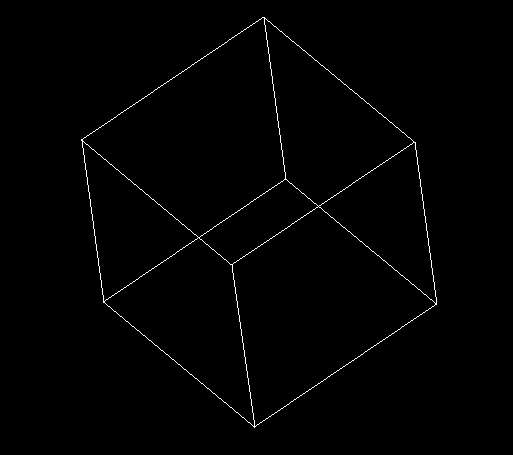
\includegraphics[width=8cm]{archivos/flatcube}
	\caption{Cubo 3D con proyección paralela}
	\label{fig:flatcube}
\end{figure}

\subsection{Refinamiento}

\begin{itemize}
	\item \textbf{Proyección cónica}: si bien la proyección paralela es muy simple de calcular en nuestro efecto, también resulta poco natural, dado que no se ajusta a la forma en la que percibimos los objetos en la realidad. Es por ello que implementamos también un proyección cónica\footnote{\url{https://es.wikipedia.org/wiki/Proyección_cónica}} muy sencilla, pero que es más cercana a la perspectiva con la que vemos en el mundo real. Para ello, haremos que el valor de las coordenadas \emph{x} e \emph{y} dependan del valor de la coordenada \emph{z}. A mayor sea \emph{z} y el objeto más lejos se encuentre, lo dibujaremos más pequeño y a menor sea \emph{z} (más cerca del origen, punto donde se sitúa la cámara), más grande se percibirá el objeto. Podemos ver un ejemplo simplificado en el código [\ref{cod:conicalperspective}]. Multiplicamos la coordenada \emph{z} por un factor definido por el usuario, para poder controlar así la fuerza de la proyección. Hay que tener en cuenta que hay que comprobar siempre que \emph{z} no sea 0, pues la división por 0 no está definida. Esta comprobación se ha omitido en el ejemplo para hacerlo más sencillo. A continuación, dividimos nuestras coordenadas \emph{x} e \emph{y} por la profundidad calculada. Si nos fijamos, no obstante, antes de realizar el cálculo, añadimos la mitad de la anchura y la altura y tras el cálculo las sustraemos. Esta operación se realiza para situar el punto de fuga de la perspectiva en el centro. Si no hiciéramos esto, los objetos, al alejarse, tenderían hacia la posición (0,0) en lugar de tender hacia el centro de la pantalla. Esto provocaría una sensación extraña, ya que veríamos los objetos alejándose hacia la esquina superior izquierda de la pantalla, lo que resulta antinatural. Este es el mismo artefacto que explicamos en el efecto anterior, y mostramos en la figura [\ref{fig:planes1}].
	\item \textbf{Múltiples objetos}: para desarrollar el efecto, añadimos la inicialización de un cubo, una figura sencilla con la que podíamos jugar libremente. Llega el momento de añadir algo más de variedad, por lo que añadimos además una pirámide y una estrella. El resultado se muestra en la figura [\ref{fig:models}].
	\item \textbf{Control del objeto}: como veíamos en el código [\ref{cod:update}], almacenamos nuestras transformaciones de traslación, rotación y escalado en un vector de \emph{Point3D} denominado \emph{transformations}. Esto nos permite manipular de un modo similar cada tipo de transformación, con lo si definimos controles para alterar las coordenadas \emph{x}, \emph{y} y \emph{z}, basta con cambiar el índice en nuestro vector de transformaciones para modificar posición, rotación o escala. Además, aprovechando que tenemos dos métodos distintos para calcular nuestra proyección, también es útil definir un control de usuario para alternarlo, así como también dar facilidad para cambiar el objeto a dibujar (almacenando nuestros objetos en un vector). En el resultado final [\ref{fig:geometry}] se muestran también las instrucciones para manipular la demo.
\end{itemize}

\begin{lstlisting}[style=C-color, caption={Cálculo de la perspectiva cónica}, label=cod:conicalperspective]
for(const Point3D& p : object.points)
{
    float depth = p.Z * depthFactor;
    
    object.projectedPoints.push_back({((p.X - halftWidth) / depth) + halftWidth,
                                     ((p.Y - halftHeight) / depth) + halftHeight});
}
\end{lstlisting}

\begin{figure}[h]
	\centering
	\begin{subfigure}[b]{0.3\textwidth}
		\centering
		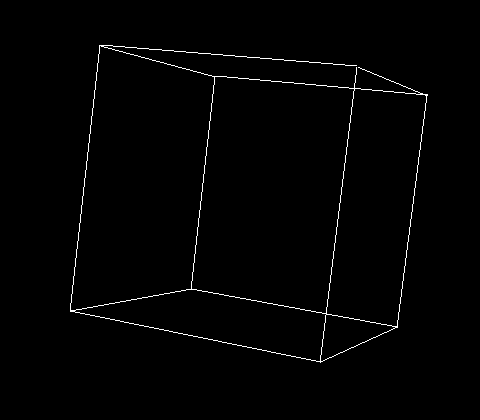
\includegraphics[width=4.5cm]{archivos/cube}
	\end{subfigure}
	\begin{subfigure}[b]{0.3\textwidth}
		\centering
		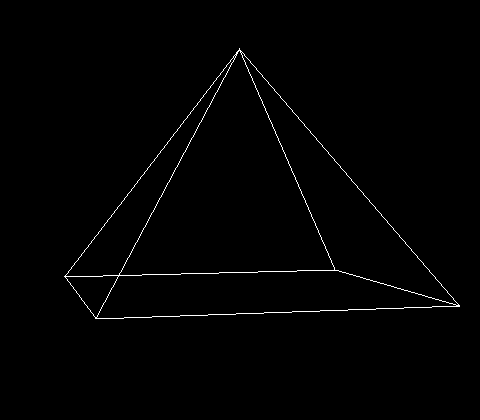
\includegraphics[width=4.5cm]{archivos/pyramid}
	\end{subfigure}
	\begin{subfigure}[b]{0.3\textwidth}
		\centering
		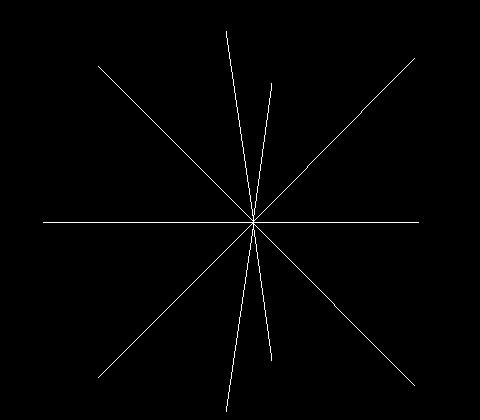
\includegraphics[width=4.5cm]{archivos/star}
	\end{subfigure}
	\caption{Distintos modelos en perspectiva}
	\label{fig:models}
\end{figure}

\subsection{Resultado}

En la figura [\ref{fig:geometry}] podemos ver un ejemplo del resultado final, donde hemos cambiado a la figura de la pirámide y la hemos rotado y escalado a voluntad. Además, tenemos disponibles las opciones adicionales para cambiar modelo y perspectiva.

\begin{figure}[h]
	\centering
	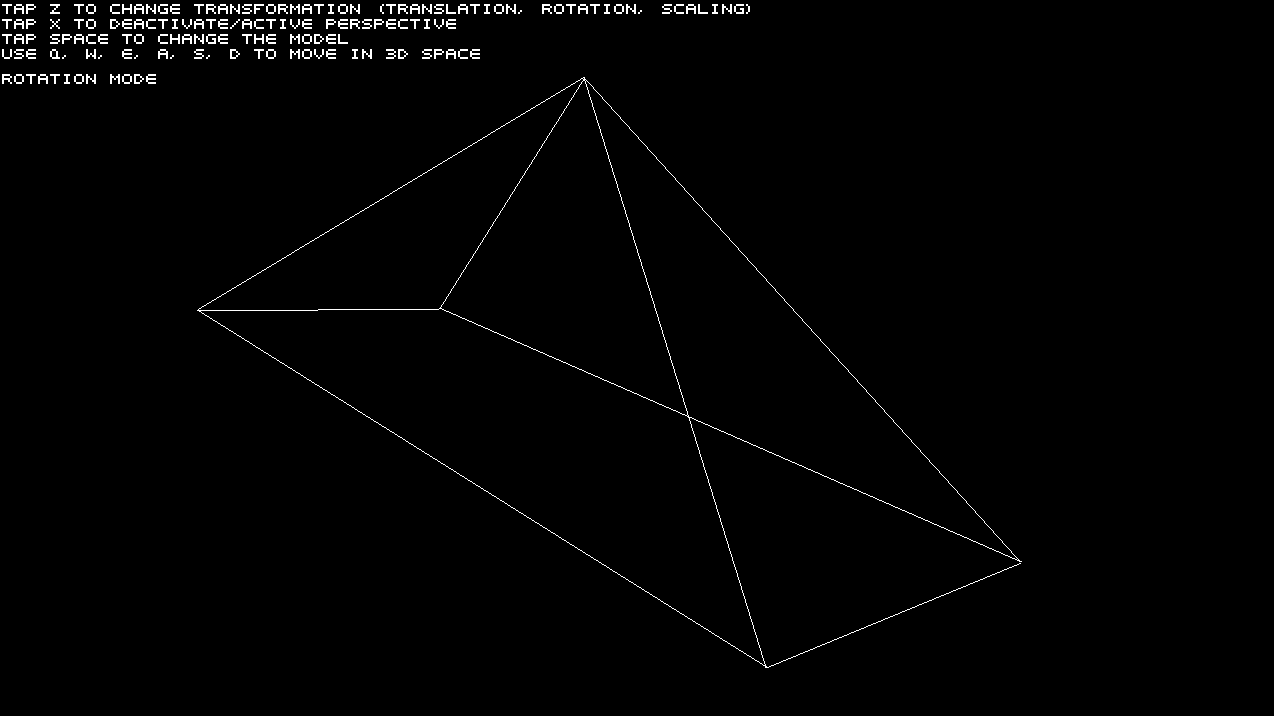
\includegraphics[width=12cm]{archivos/geometry}
	\caption{Pirámide rotada y escalada}
	\label{fig:geometry}
\end{figure}
